\documentclass{article}

\usepackage{graphicx}
\usepackage{amsmath}
\usepackage{fancyhdr}
\usepackage{float}
\usepackage[sorting=none]{biblatex}
\usepackage[margin=1in]{geometry}
\usepackage[font={small,it}]{caption}
\usepackage{placeins}
\usepackage{xepersian}

%\DeclareMathOperator*{\btie}{\bowtie}
\addbibresource{bibliography.bib}
\settextfont[Scale=1.2]{B-NAZANIN.TTF}
\setlatintextfont[Scale=1]{Times New Roman}
\renewcommand{\baselinestretch}{1.5}
\pagestyle{fancy}
\fancyhf{}
\rhead{تکلیف اول آزمایشگاه شبکه ‌های کامپیوتری}
\lhead{\thepage}
\rfoot{علیرضا ابره فروش}
\lfoot{9816603}
\renewcommand{\headrulewidth}{1pt}
\renewcommand{\footrulewidth}{1pt}

\begin{document}
\begin{titlepage}
\begin{center}

\includegraphics[width=0.4\textwidth]{figures/IUT Logo.png}\\
        
\LARGE
\textbf{دانشگاه صنعتی اصفهان}\\
\textbf{دانشکده مهندسی برق و کامپیوتر}\\
        
\vfill
        
\huge
\textbf{عنوان: تکلیف چهارم درس ریزپردازنده}\\
        
\vfill
        
\LARGE
\textbf{نام و نام خانوادگی: علیرضا ابره فروش}\\
\textbf{شماره دانشجویی: 9816603}\\
\textbf{نیم\,سال تحصیلی: پاییز 1400}\\
\textbf{مدرّس: دکتر عارف کریمی افشار}\\
\end{center}
\end{titlepage}


%\tableofcontents
\newpage



\section{}
\subsection{}
\begin{figure}[H]
    \centering
    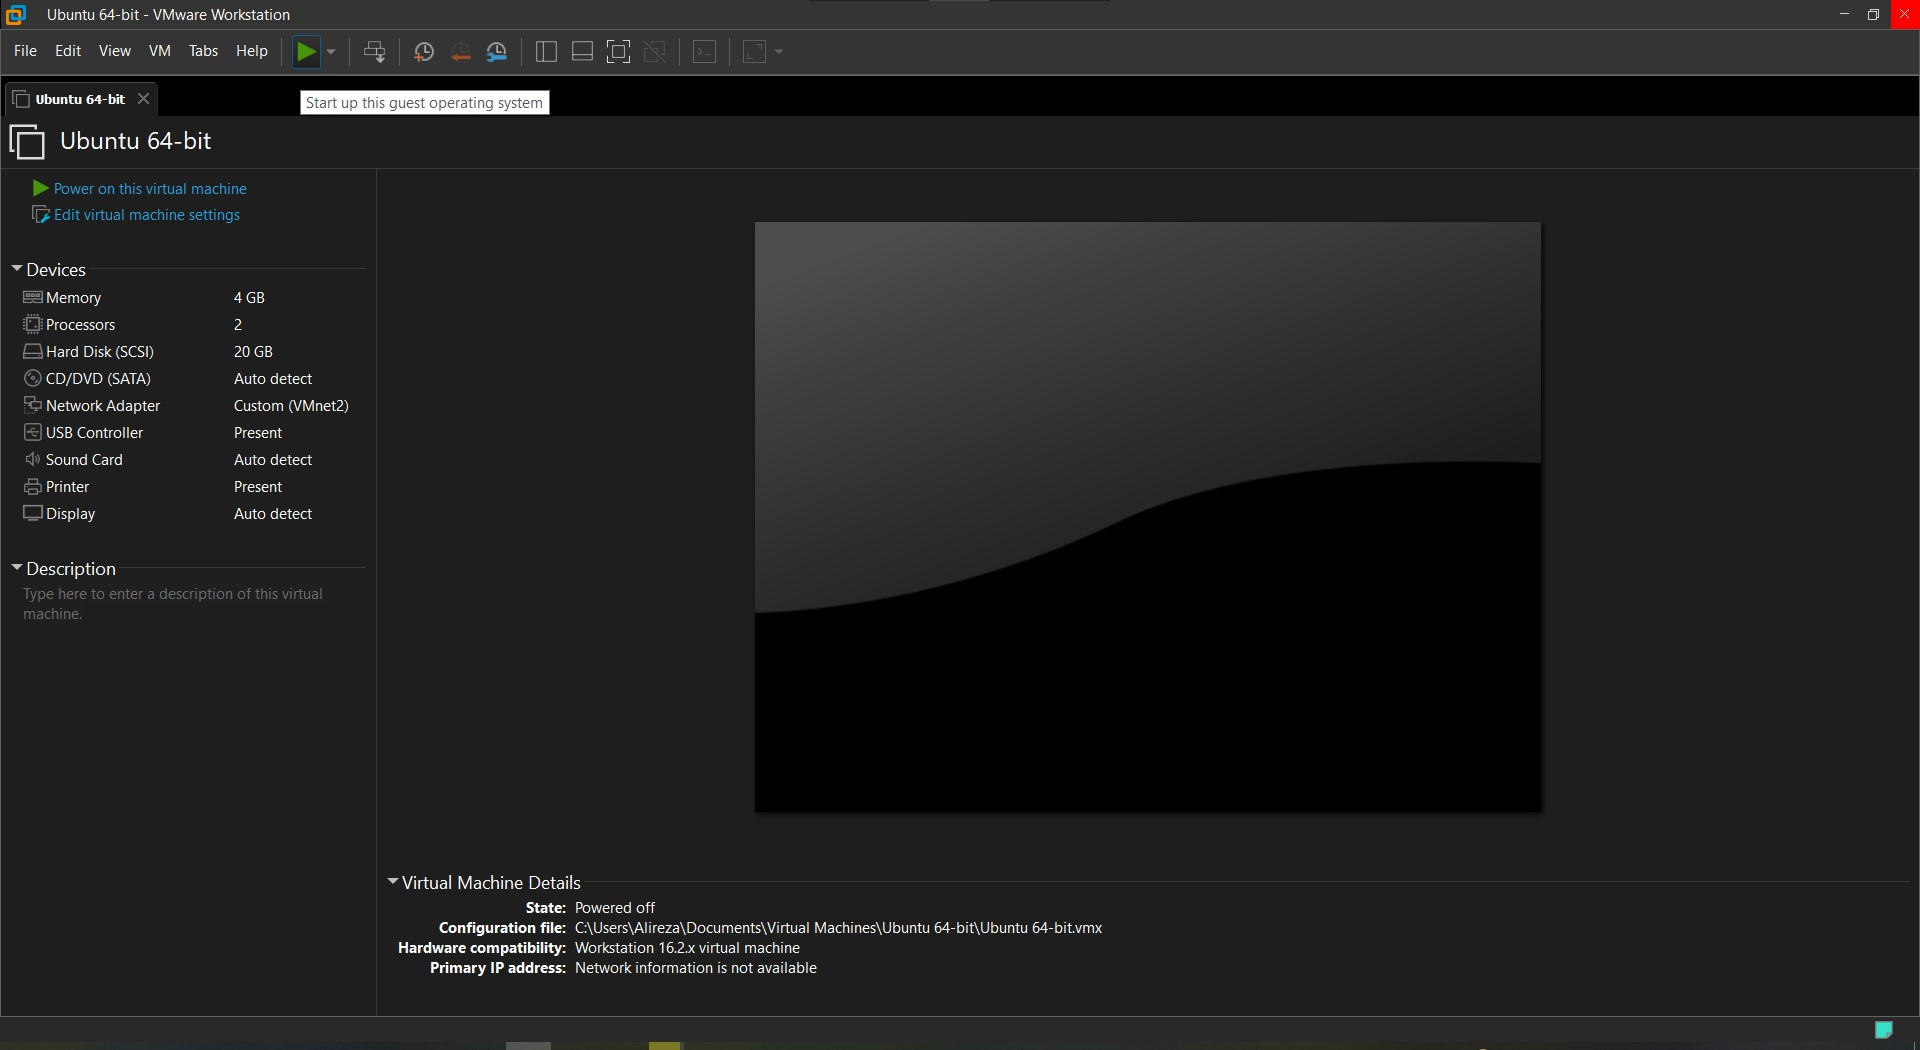
\includegraphics[width=1.0\textwidth]{figures/1a.jpg}
    \caption
	{
\lr{VMware Workstation}
	}
    \label{fig:fig1}
\end{figure}
ماشین مجازی را به این طریق روشن می‌کنیم.

\subsection{}
\begin{figure}[H]
    \centering
    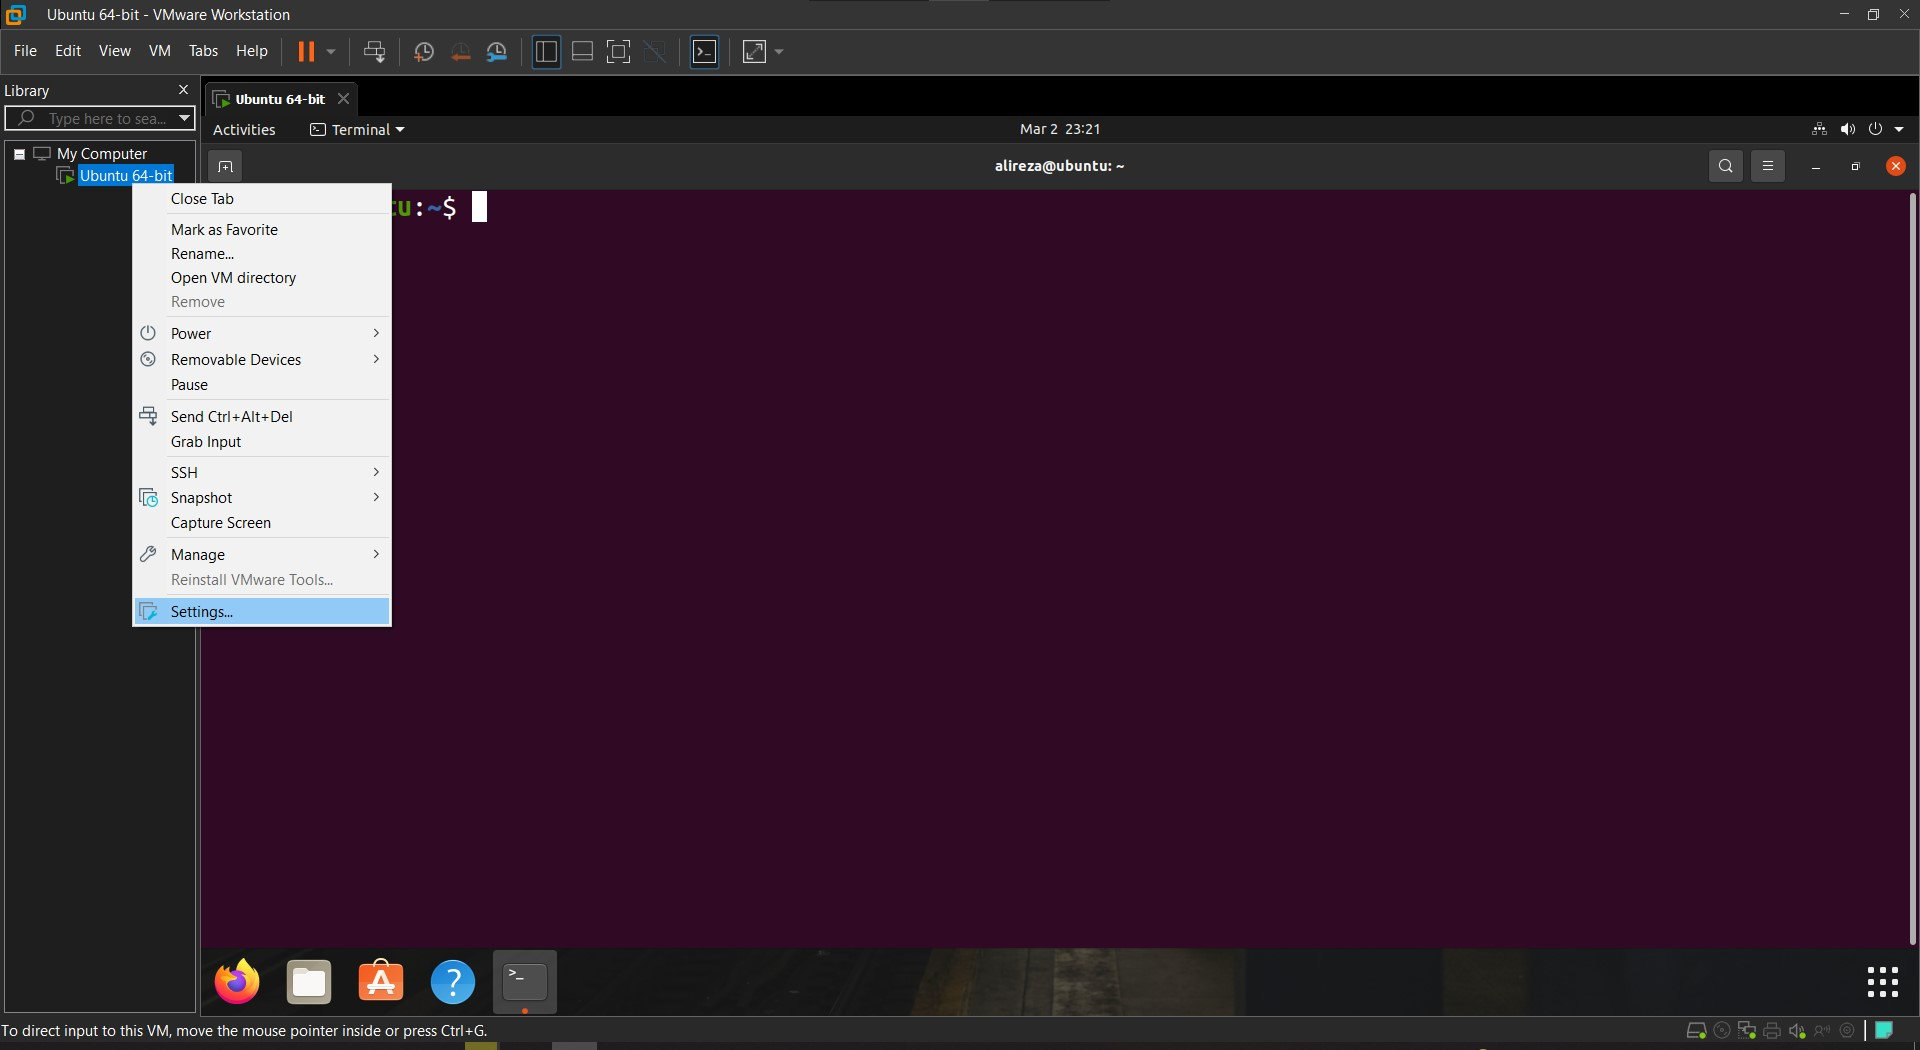
\includegraphics[width=1.0\textwidth]{figures/2a.jpg}
    \caption
	{
\lr{Virtual Machine Settings}
	}
    \label{fig:fig1}
\end{figure}
ابتدا وارد تنظیمات شبکه ماشین مجازی می‌شویم.
\begin{figure}[H]
    \centering
    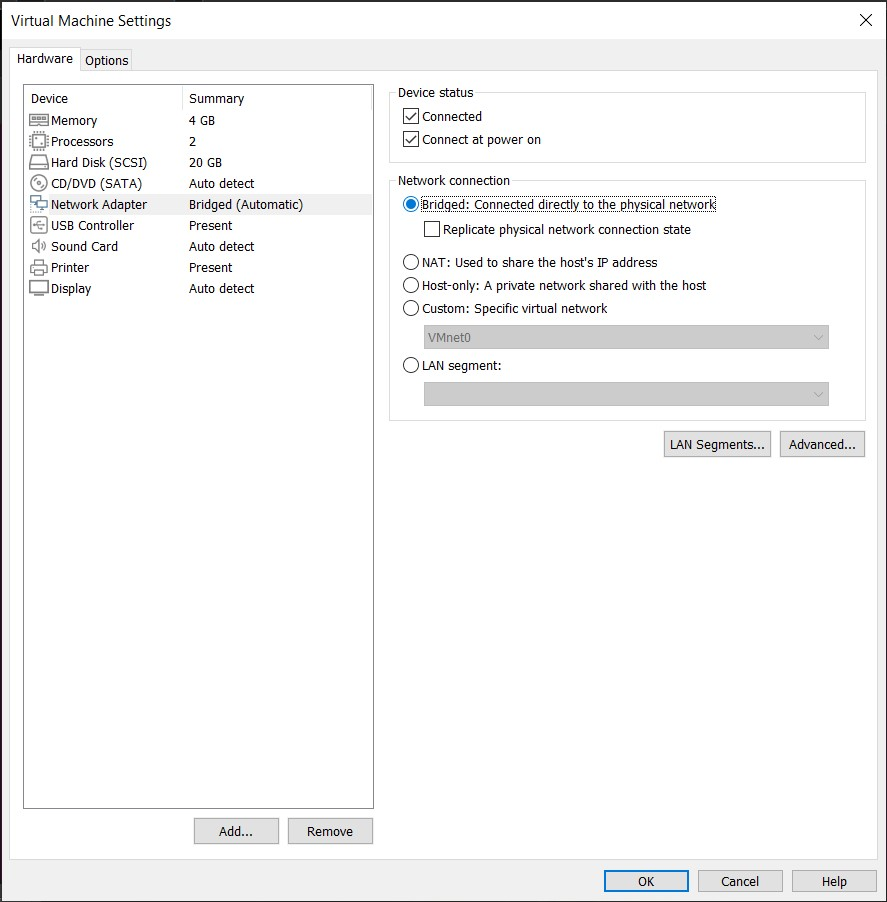
\includegraphics[width=1.0\textwidth]{figures/2b.jpg}
    \caption
	{
\lr{Bridged Network Connection}
	}
    \label{fig:fig1}
\end{figure}
سپس حالت شبکه را روی \lr{Bridged} قرار می‌دهیم.
\begin{figure}[H]
    \centering
    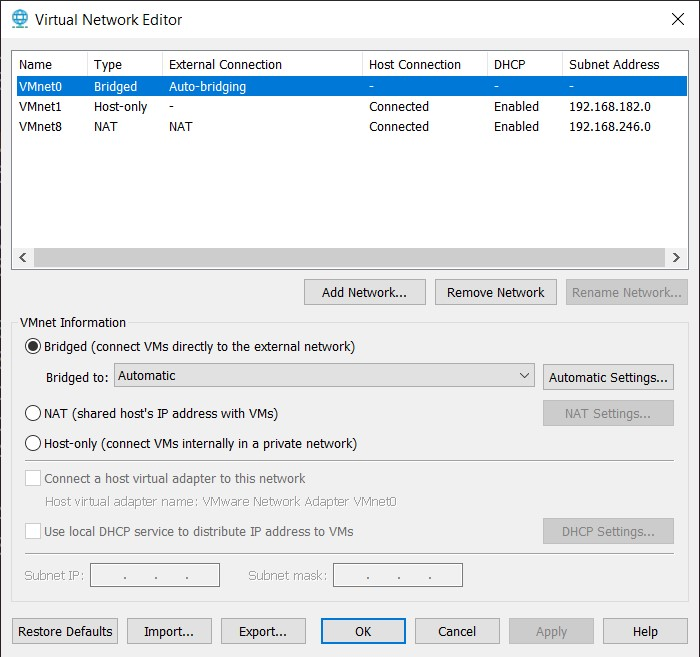
\includegraphics[width=1.0\textwidth]{figures/2b1.jpg}
    \caption
	{
\lr{Virtual Network Editor(Bridged)}
	}
    \label{fig:fig1}
\end{figure}
این شبکه در محدوده‌ی \lr{VMnet0} است.
\begin{figure}[H]
    \centering
    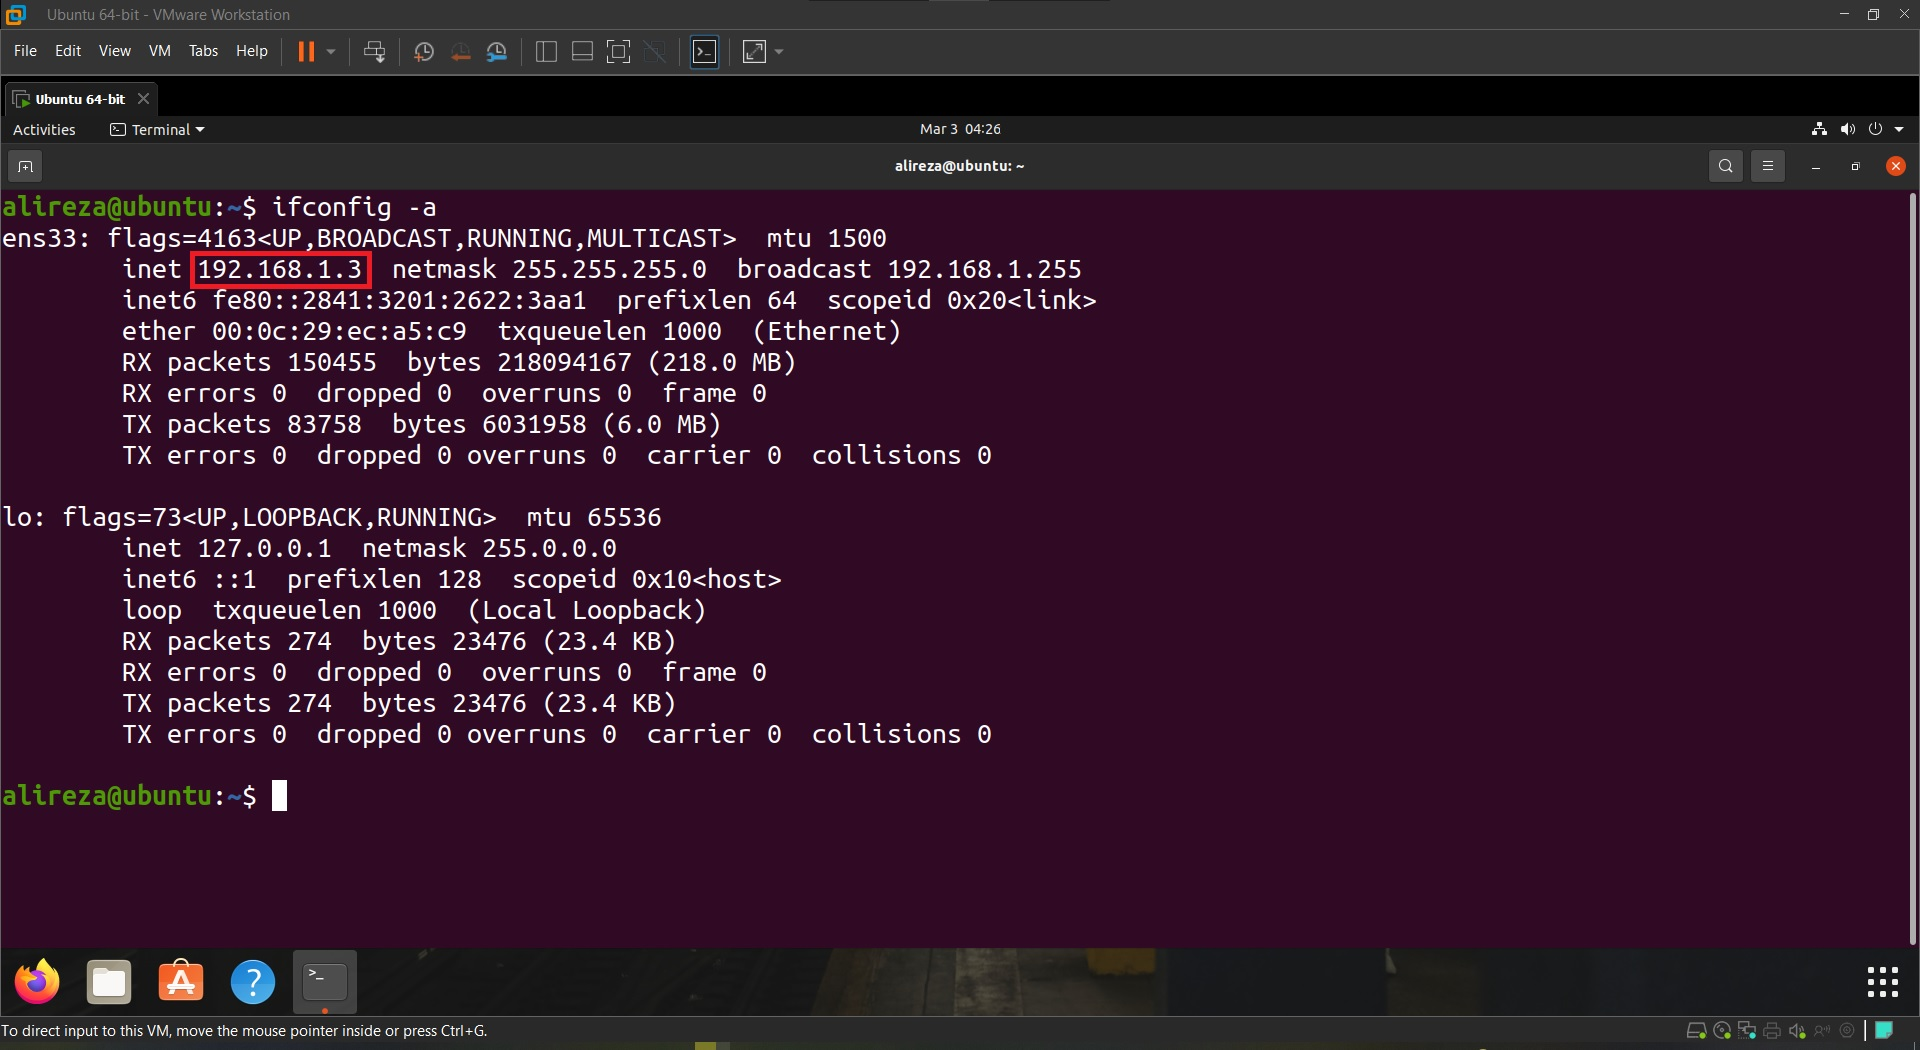
\includegraphics[width=1.0\textwidth]{figures/2c.jpg}
    \caption
	{
خروجی دستور \lr{ifconfig -a} در ماشین مجازی
	}
    \label{fig:fig1}
\end{figure}

\begin{figure}[H]
    \centering
    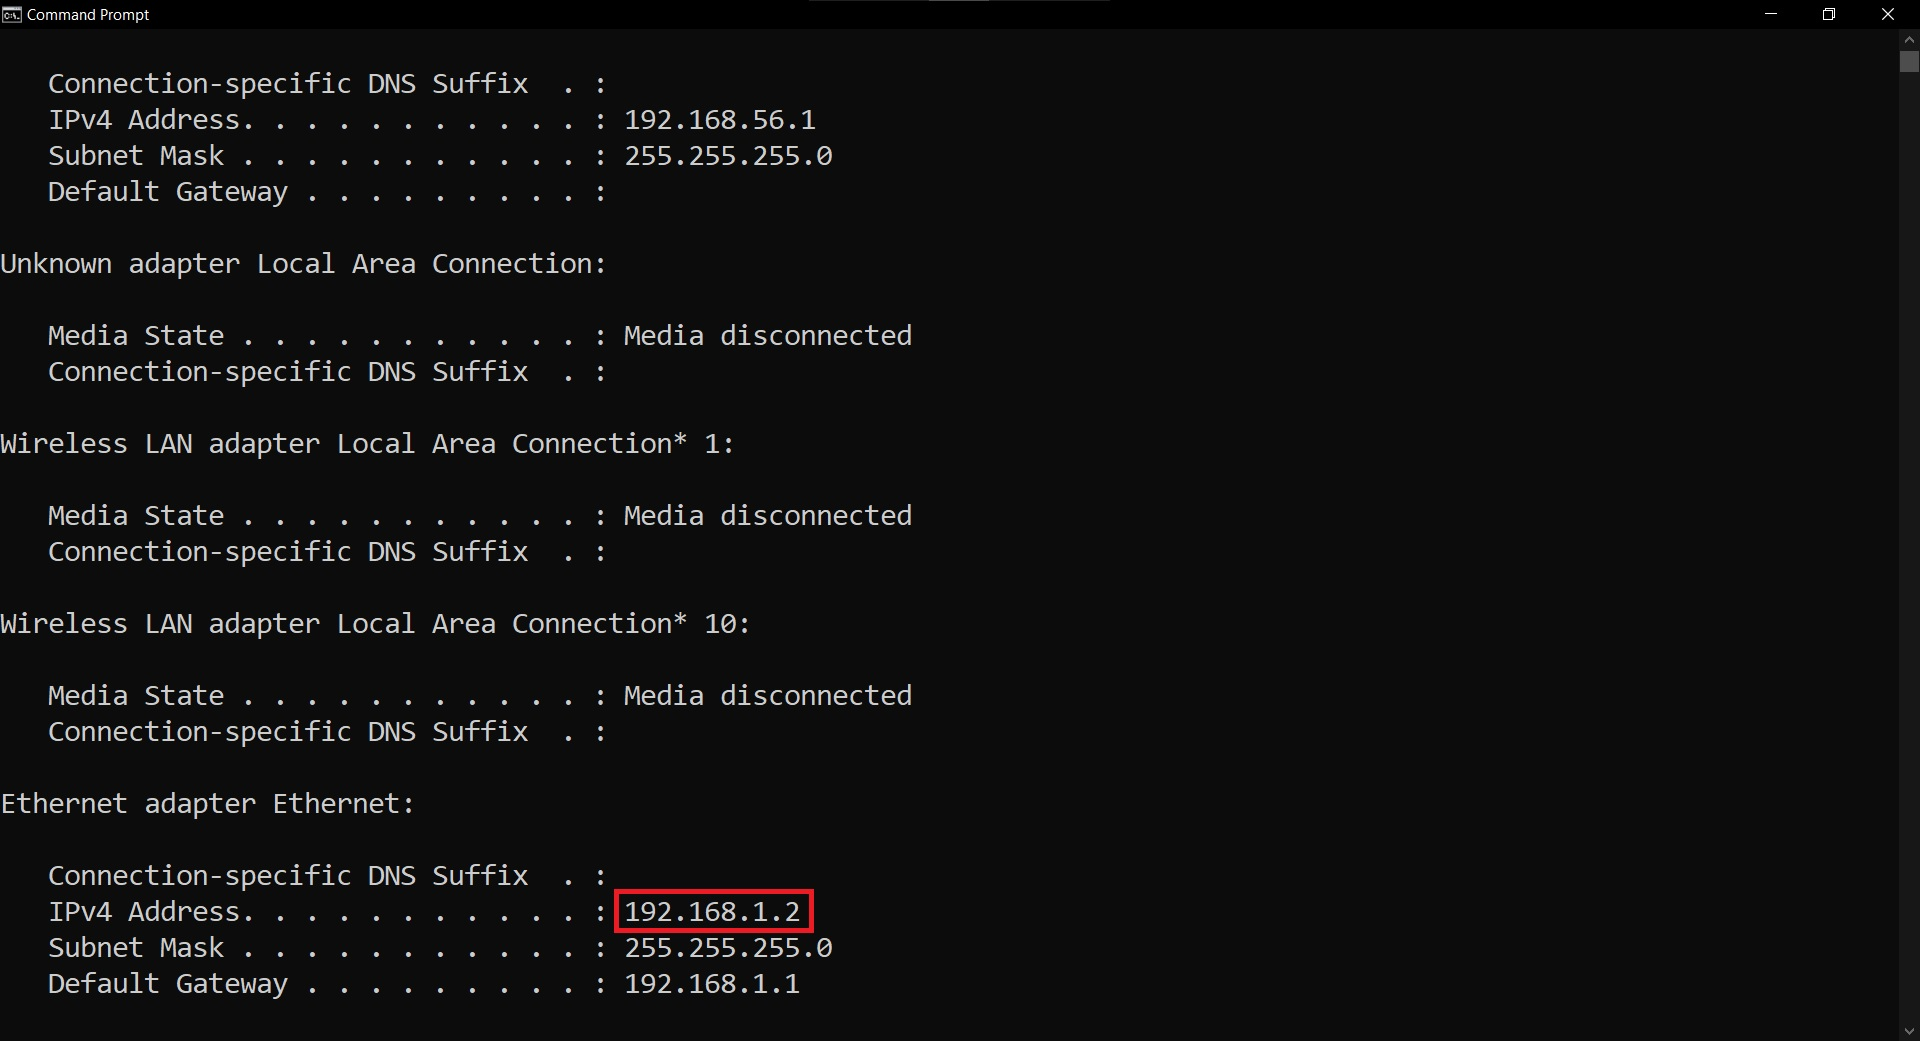
\includegraphics[width=1.0\textwidth]{figures/2d.jpg}
    \caption
	{
خروجی دستور \lr{ipconfig} در میزبان
	}
    \label{fig:fig1}
\end{figure}
رنج آدرس‌های آی‌پی در ماشین مجازی و در میزبان برابر است. چون در حالت \lr{Bridged} ماشین مجازی از طریق کارت شبکه سیستم اصلی به شبکه محلی متصل می‌شود. در این روش کارت شبکه مجازی در ماشین مجازی به کارت شبکه فیزیکی متصل شده و می‌تواند ماشین مجازی را همانند یک سیستم مستقل به شبکه محلی متصل نماید. در صورتی که در سیستم اصلی چند کارت شبکه وجود داشته باشد، در ماشین(های) مجازی می‌توان هر کارت شبکه مجازی را با هرکدام از کارت شبکه‌های سیستم اصلی \lr{Bridge} نمود. در این حالت باید آدرس آی‌پی‌های ماشین مجازی و کارت شبکه فیزیکی که با آن \lr{Bridge} شده است در یک رنج باشند تا بتوانند ارتباط لایه 2 درستی با یکدیگر برقرار نمایند.
\subsection{}
\begin{figure}[H]
    \centering
    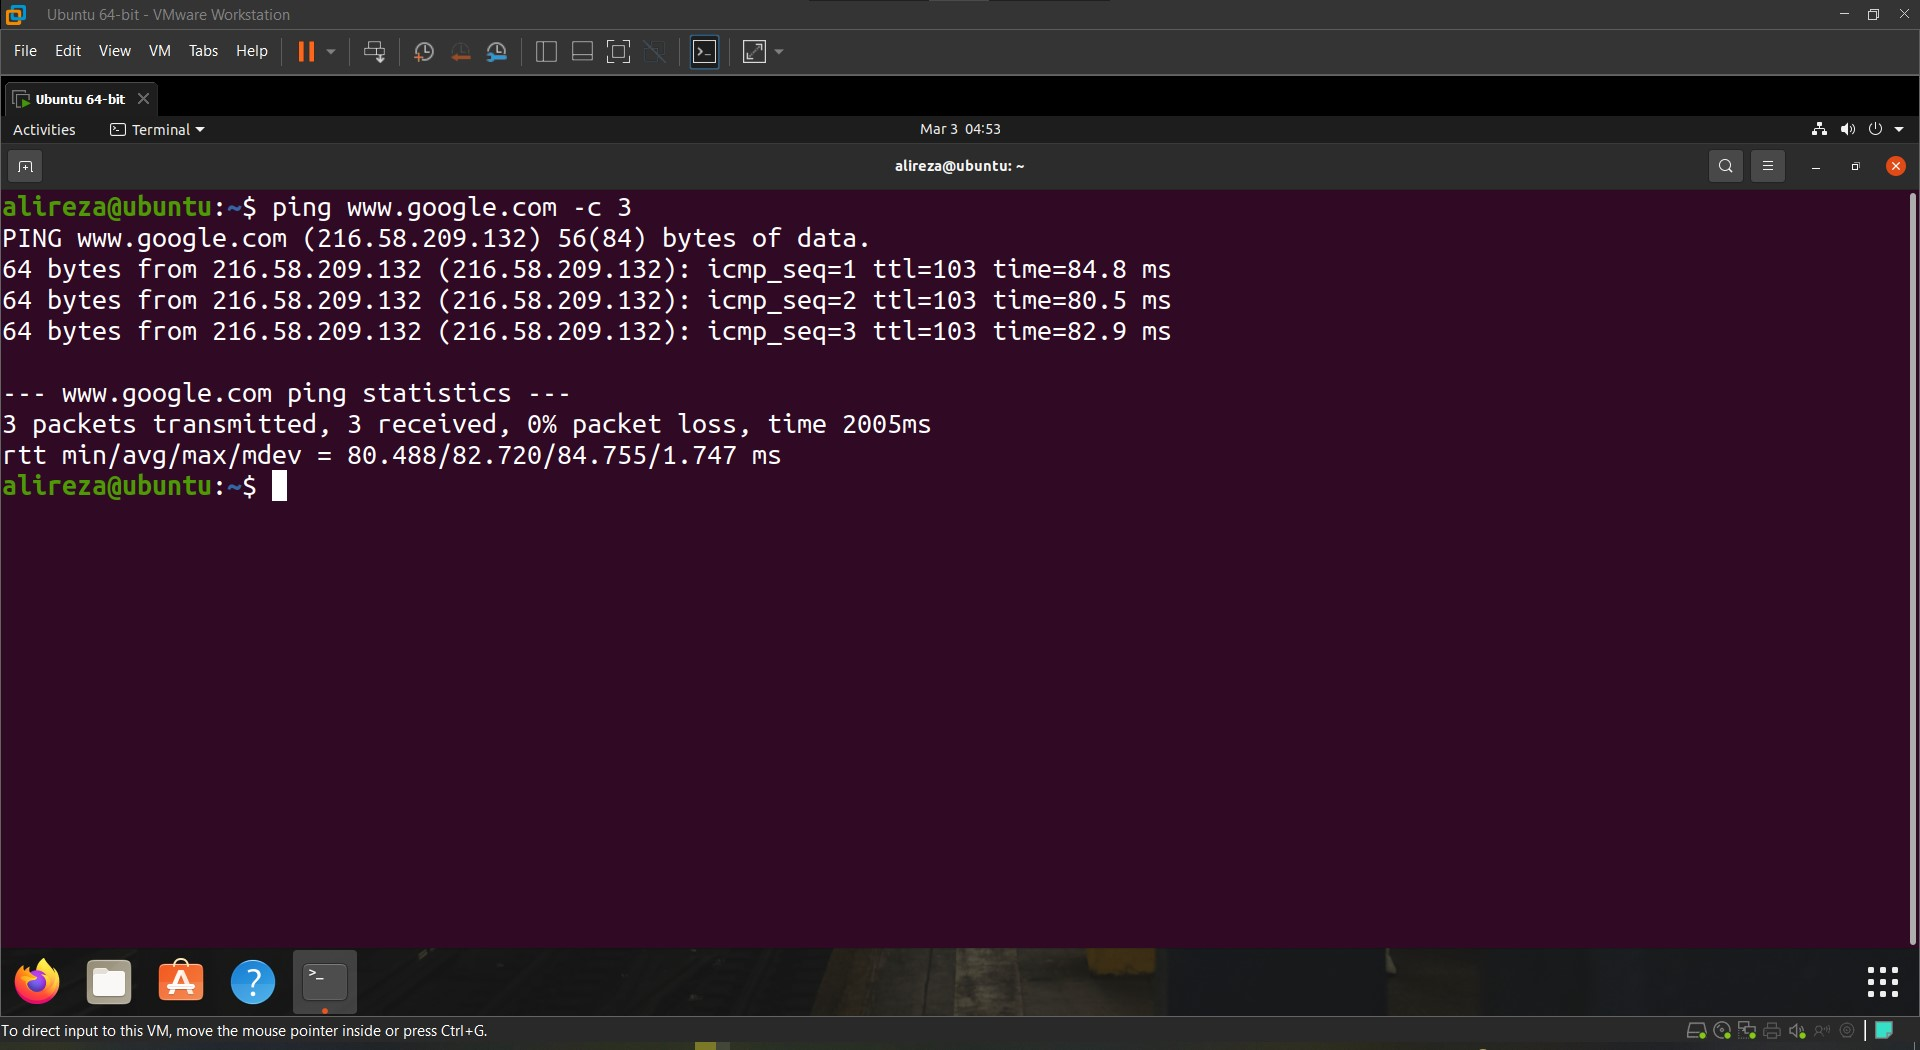
\includegraphics[width=1.0\textwidth]{figures/3a.jpg}
    \caption
	{
\lr{ping www.google.com -c 3}
	}
    \label{fig:fig1}
\end{figure}
خروجی دستور \lr{ping www.google.com -c 3} نشان می‌دهد که اتصال به اینترنت برقرار است.
\begin{figure}[H]
    \centering
    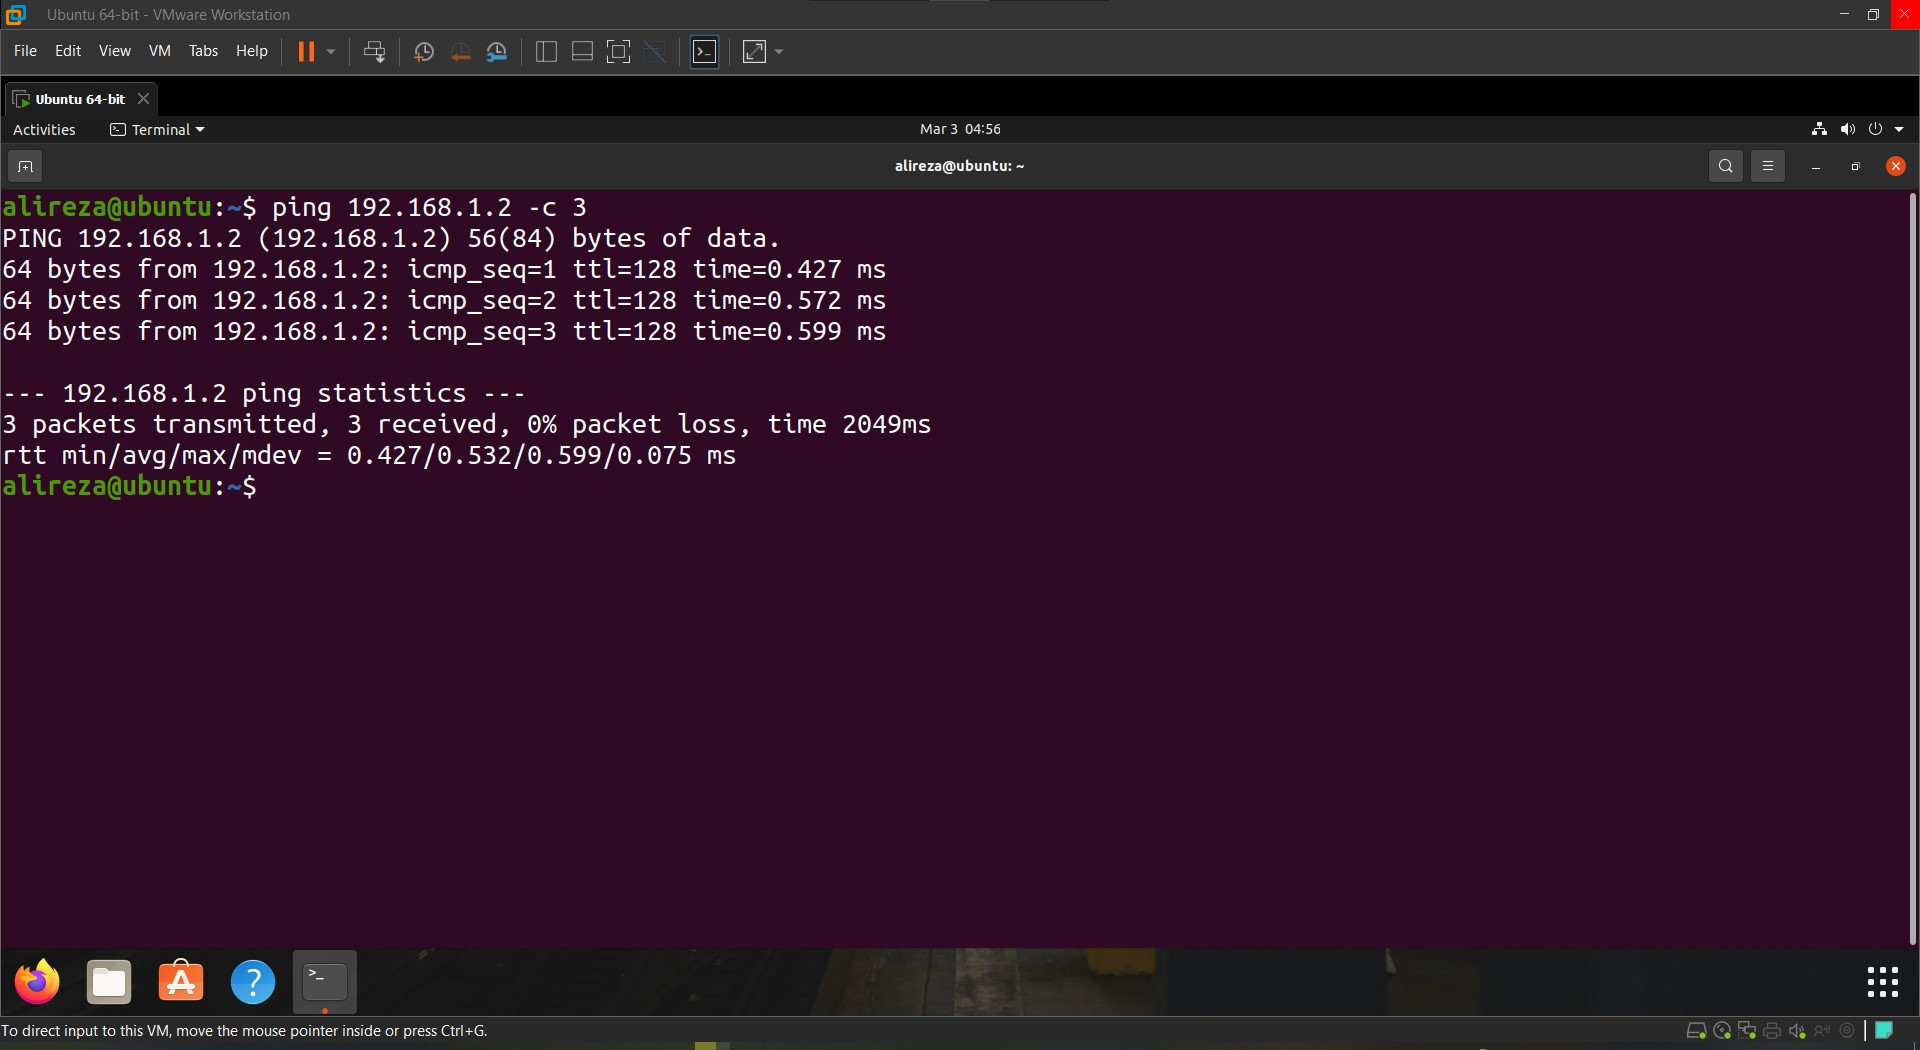
\includegraphics[width=1.0\textwidth]{figures/3b.jpg}
    \caption
	{
\lr{ping 192.168.1.2 -c 3}
	}
    \label{fig:fig1}
\end{figure}
خروجی دستور \lr{ping 192.168.1.2 -c 3} نشان می‌دهد که ماشین مجازی به میزبان دسترسی دارد که با توجه به ویژگی‌های مذکور در قسمت‌های قبل درباره‌ی شبکه در حالت \lr{Bridged} مورد انتظار است.
\begin{figure}[H]
    \centering
    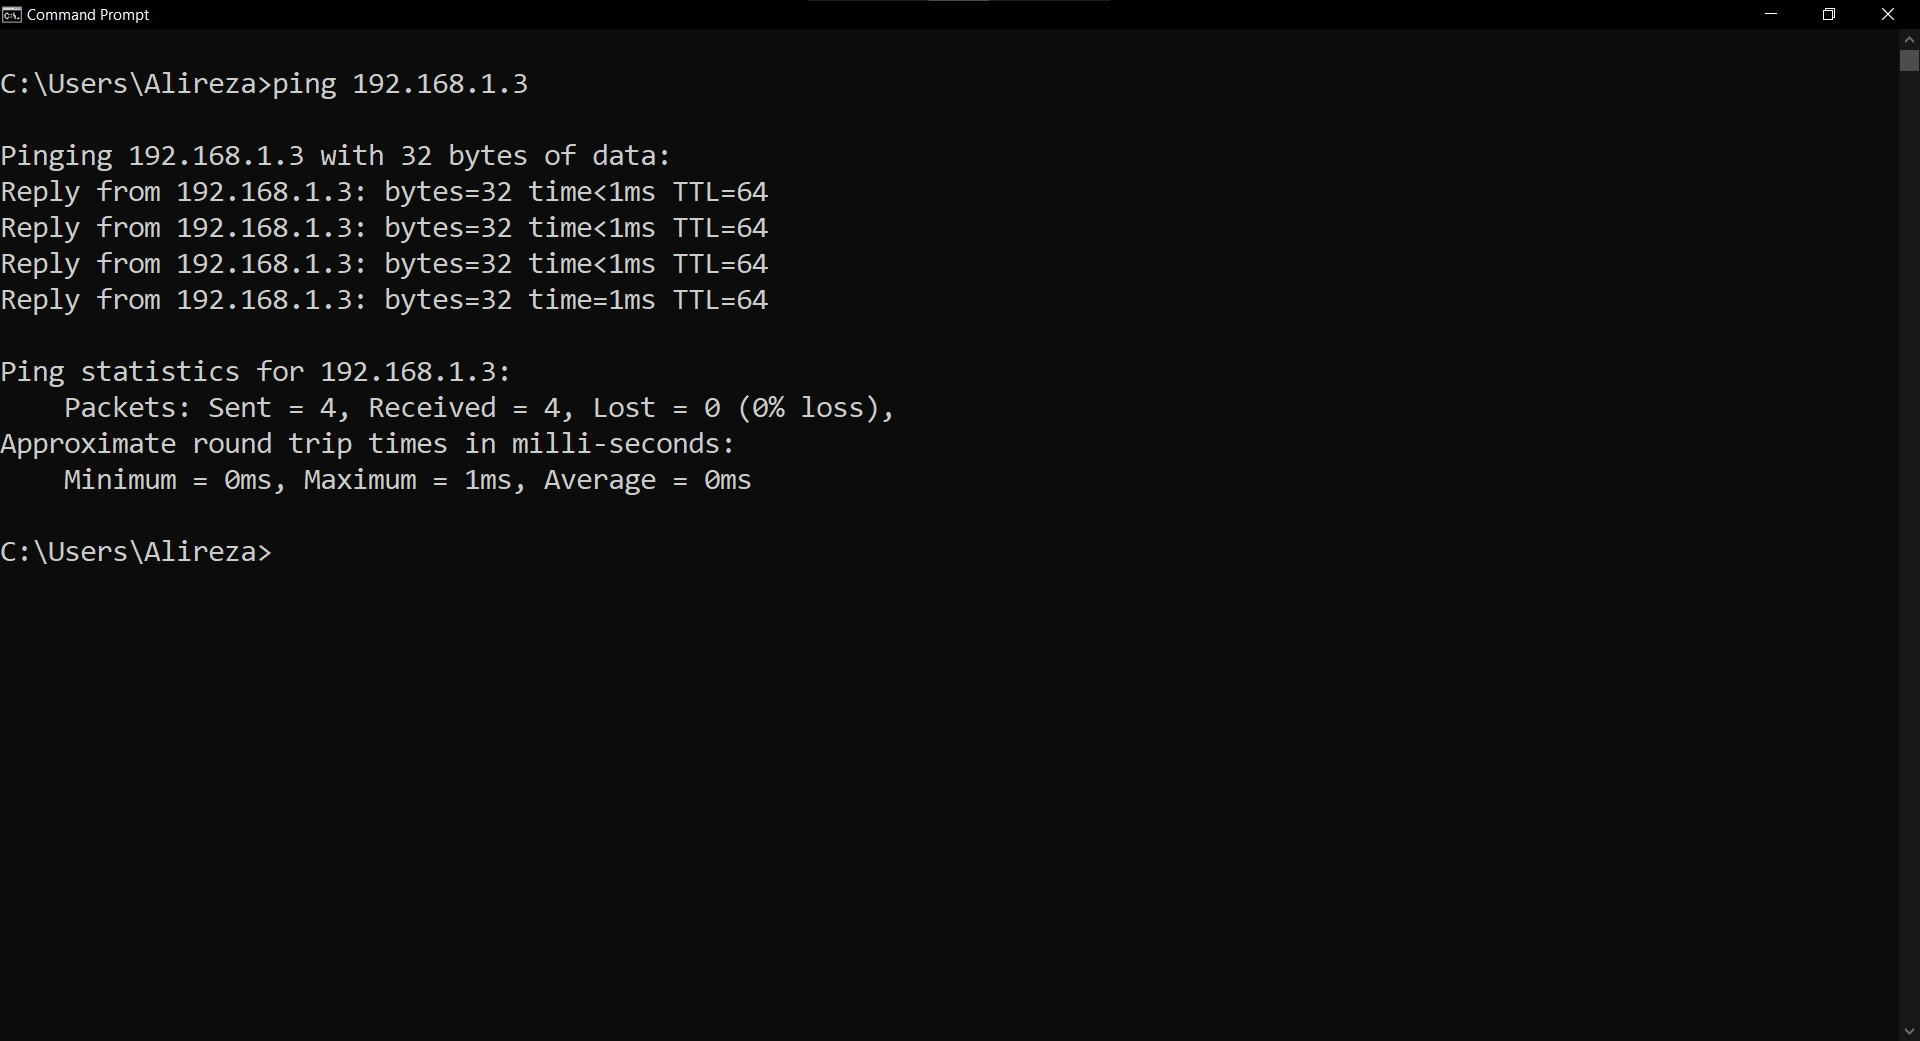
\includegraphics[width=1.0\textwidth]{figures/3c.jpg}
    \caption
	{
\lr{ping 192.168.1.3}
	}
    \label{fig:fig1}
\end{figure}
با توجه به اینکه سیستم میزبان به ماشین‌های مجازی به میزبانی خودش صرف نظر از نوع شبکه‌ی آن‌ها دسترسی دارد پس باید پینگ موفق باشد.
\subsection{}
\begin{figure}[H]
    \centering
    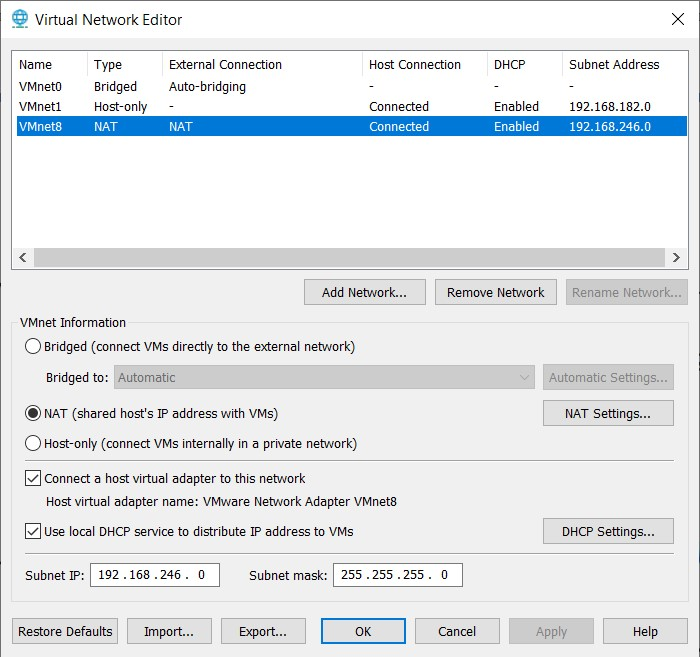
\includegraphics[width=1.0\textwidth]{figures/4a.jpg}
    \caption
	{
\lr{Virtual Network Editor(NAT)}
	}
    \label{fig:fig1}
\end{figure}
می‌بینیم که رنجِ آی‌پیِ \lr{NAT}، برابر \lr{192.168.246} است.
\begin{figure}[H]
    \centering
    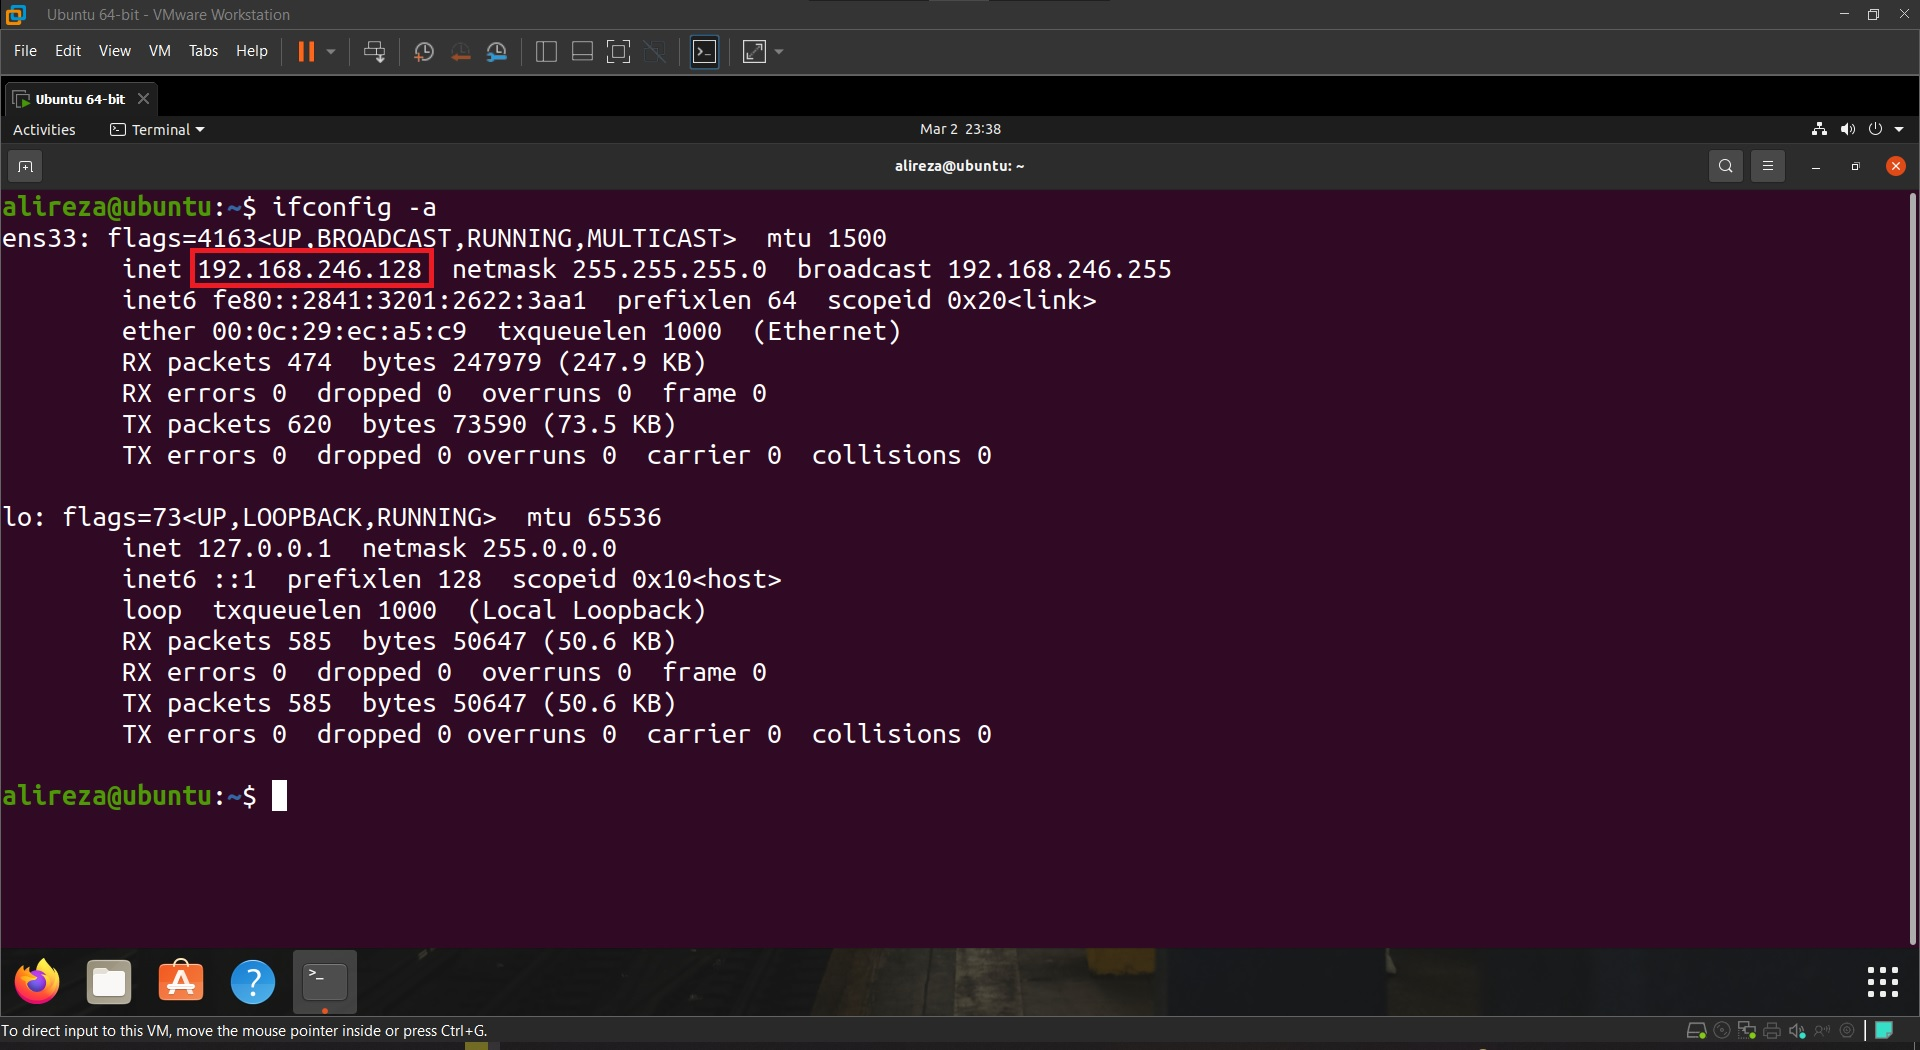
\includegraphics[width=1.0\textwidth]{figures/4b.jpg}
    \caption
	{
\lr{ifconfig -a}
	}
    \label{fig:fig1}
\end{figure}
این آدرس در محدوده‌ی \lr{VMnet8} است.
\begin{figure}[H]
    \centering
    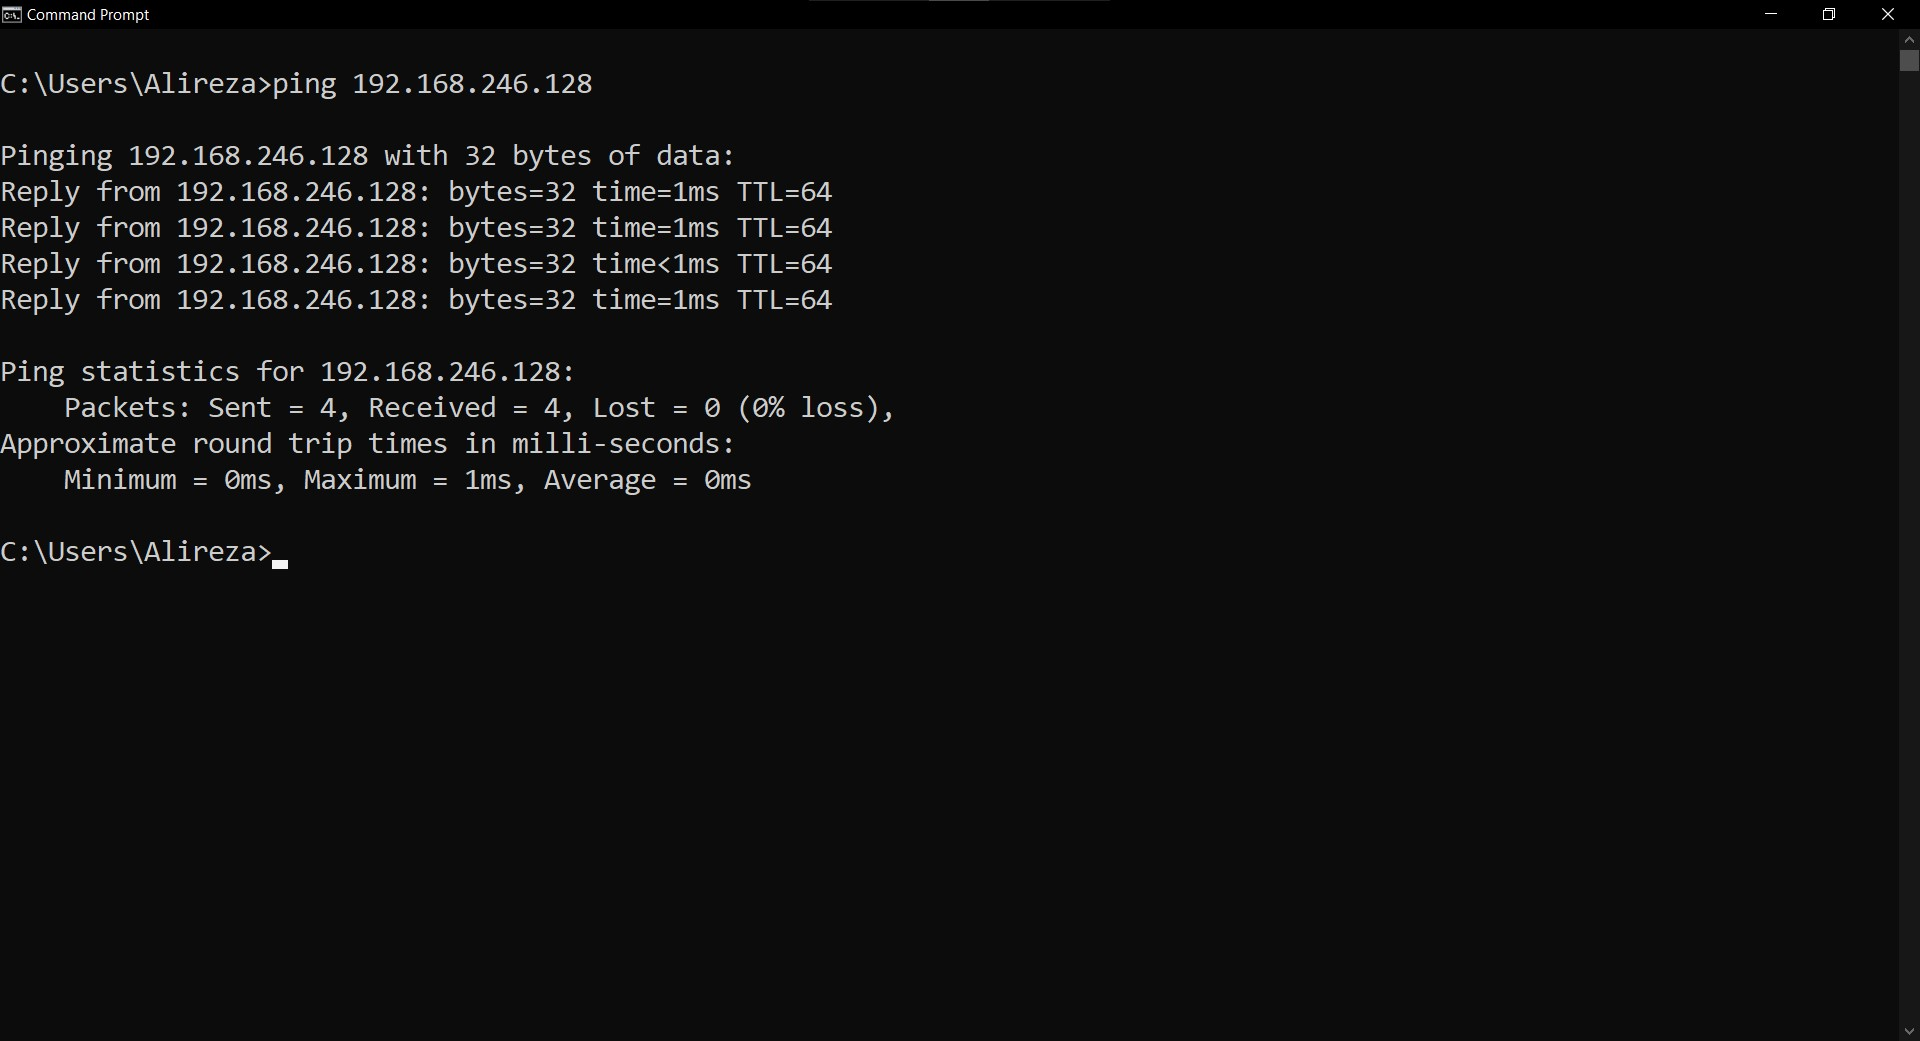
\includegraphics[width=1.0\textwidth]{figures/4c.jpg}
    \caption
	{
\lr{ping 192.168.246.128}
	}
    \label{fig:fig1}
\end{figure}
میزبان در هر سه حالت به سیستم مجازی دسترسی دارد.


\subsection{}
\begin{figure}[H]
    \centering
    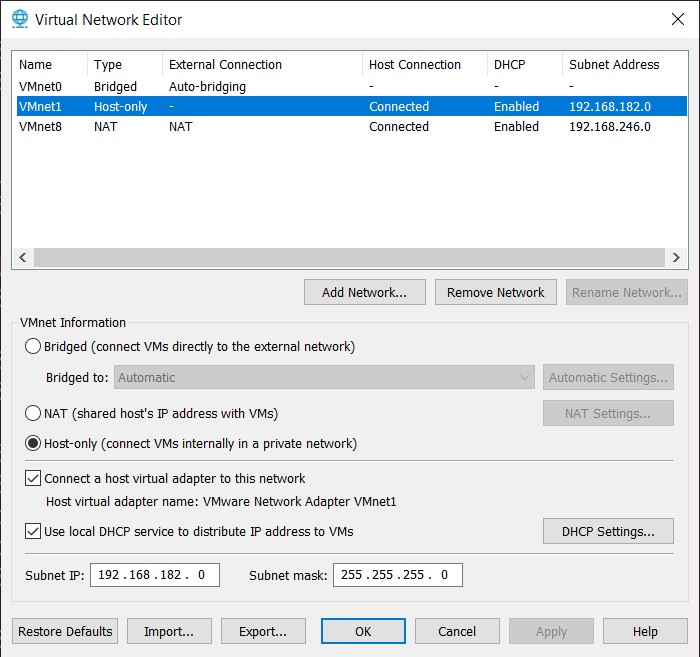
\includegraphics[width=1.0\textwidth]{figures/5a.jpg}
    \caption
	{
\lr{Virtual Network Editor(Host-only)}
	}
    \label{fig:fig1}
\end{figure}
می‌بینیم که رنجِ آی‌پیِ \lr{Host-only}، برابر \lr{192.168.182} است.
\subsection{}
\begin{figure}[H]
    \centering
    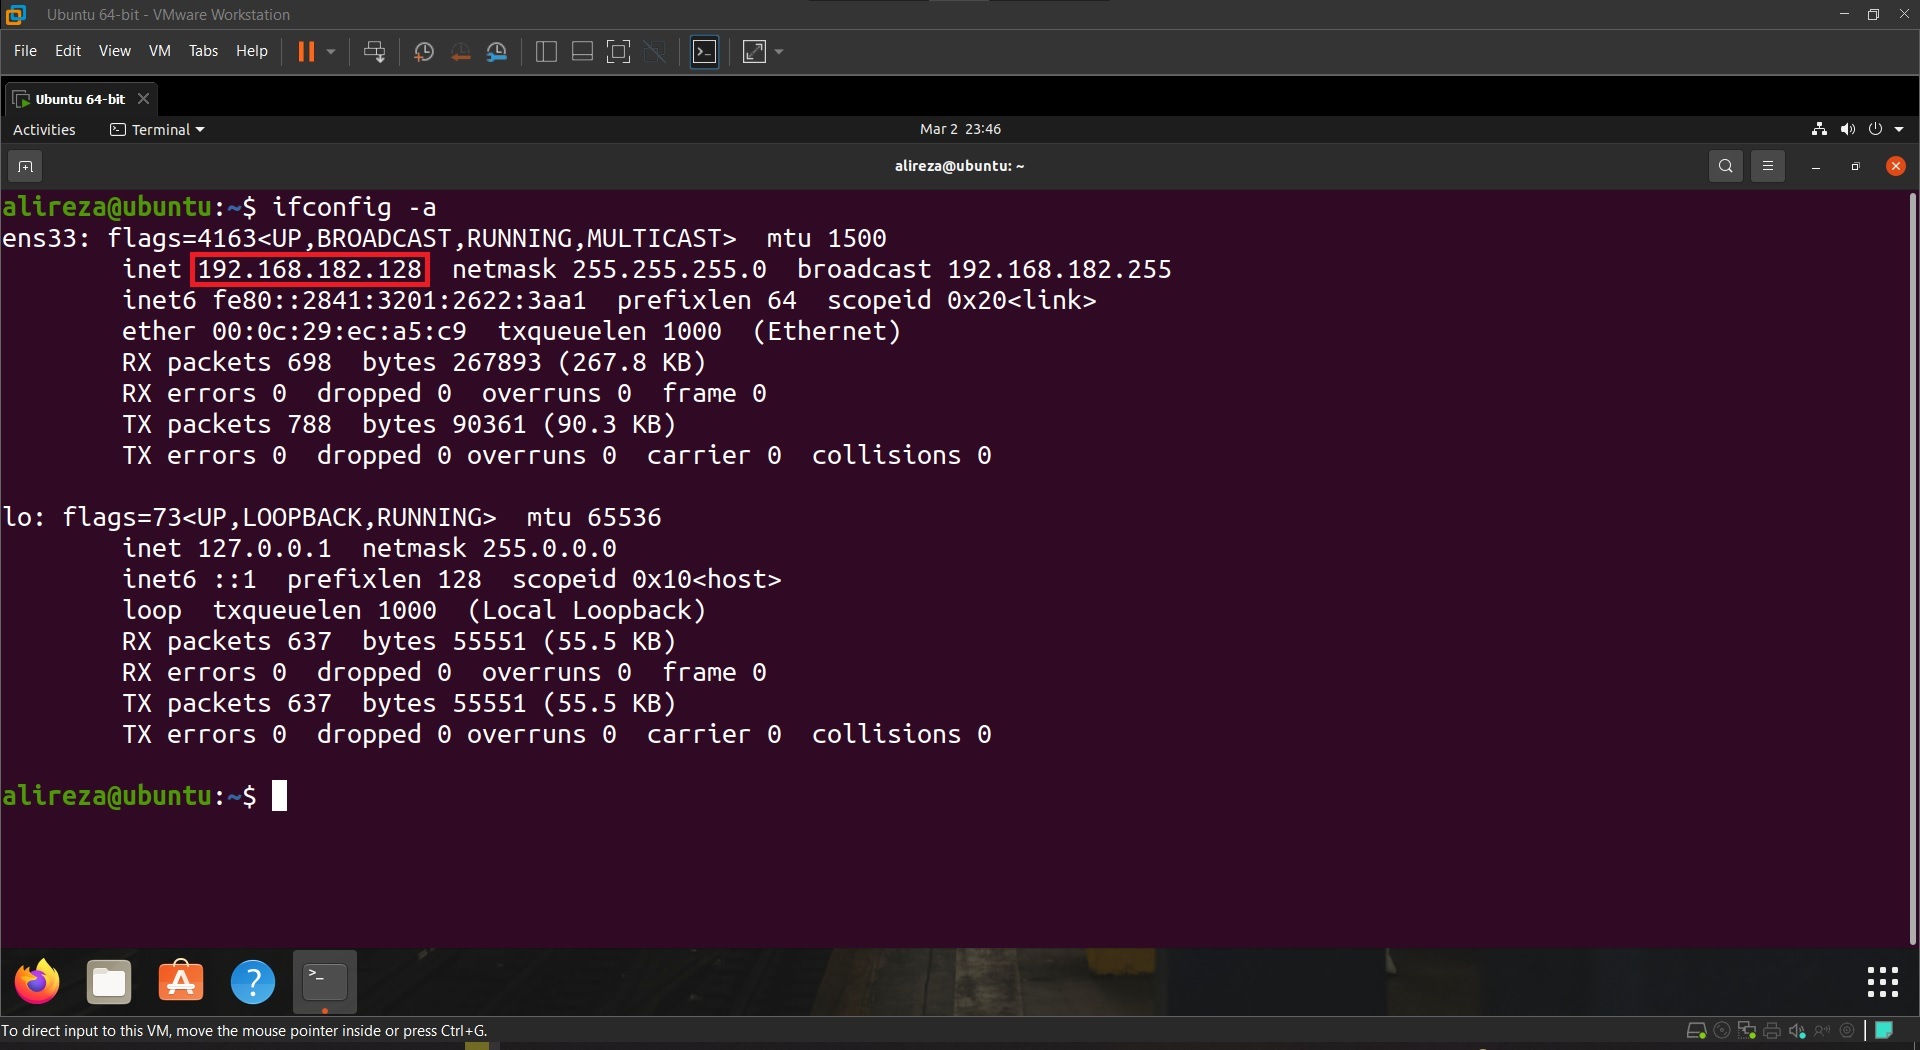
\includegraphics[width=1.0\textwidth]{figures/5b.jpg}
    \caption
	{
\lr{ifconfig -a}
	}
    \label{fig:fig1}
\end{figure}
این آدرس در محدوده‌ی \lr{VMnet1} است. چون به طور پیش‌فرض \lr{Host-only} روی \lr{VMnet1} کانفیگ شده است.

\subsection{}
\begin{figure}[H]
    \centering
    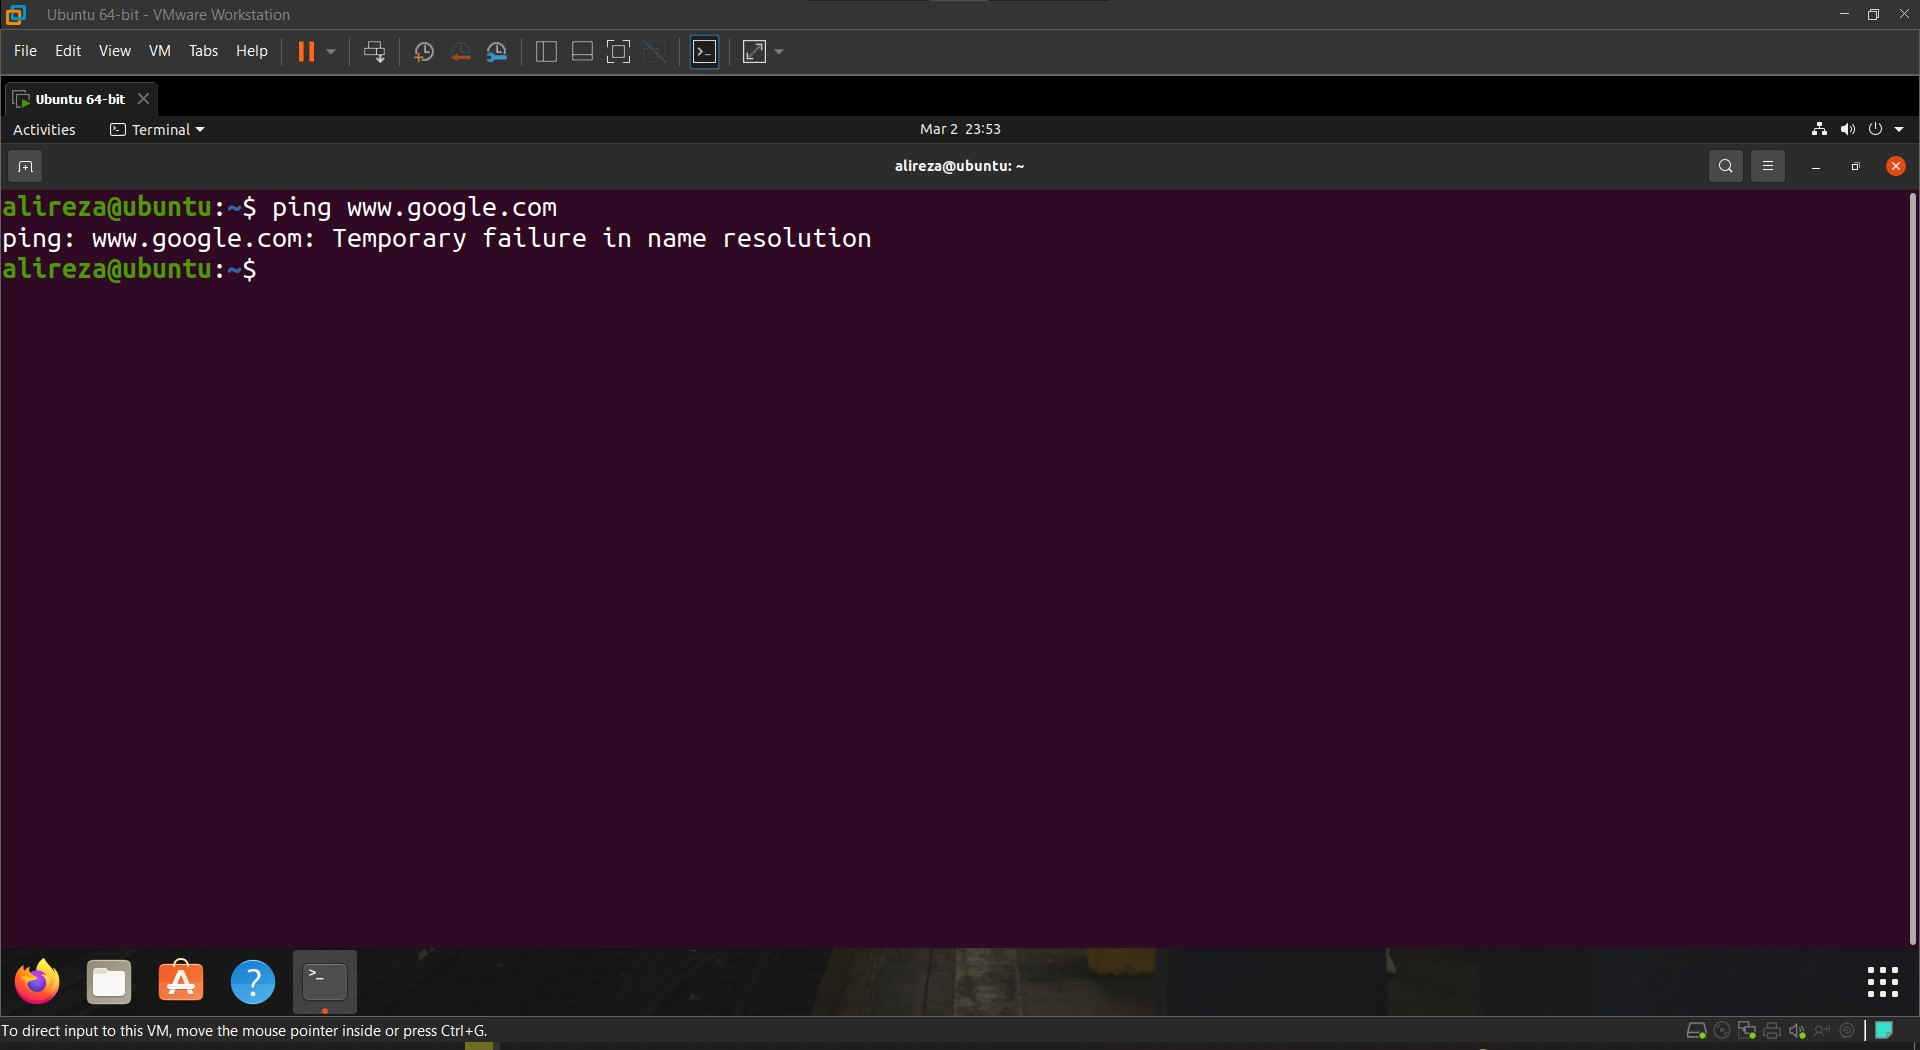
\includegraphics[width=1.0\textwidth]{figures/6a.jpg}
    \caption
	{
\lr{ping www.google.com}
	}
    \label{fig:fig1}
\end{figure}
در حالت \lr{Host-only} اتصال به اینترنت نداریم.
\begin{figure}[H]
    \centering
    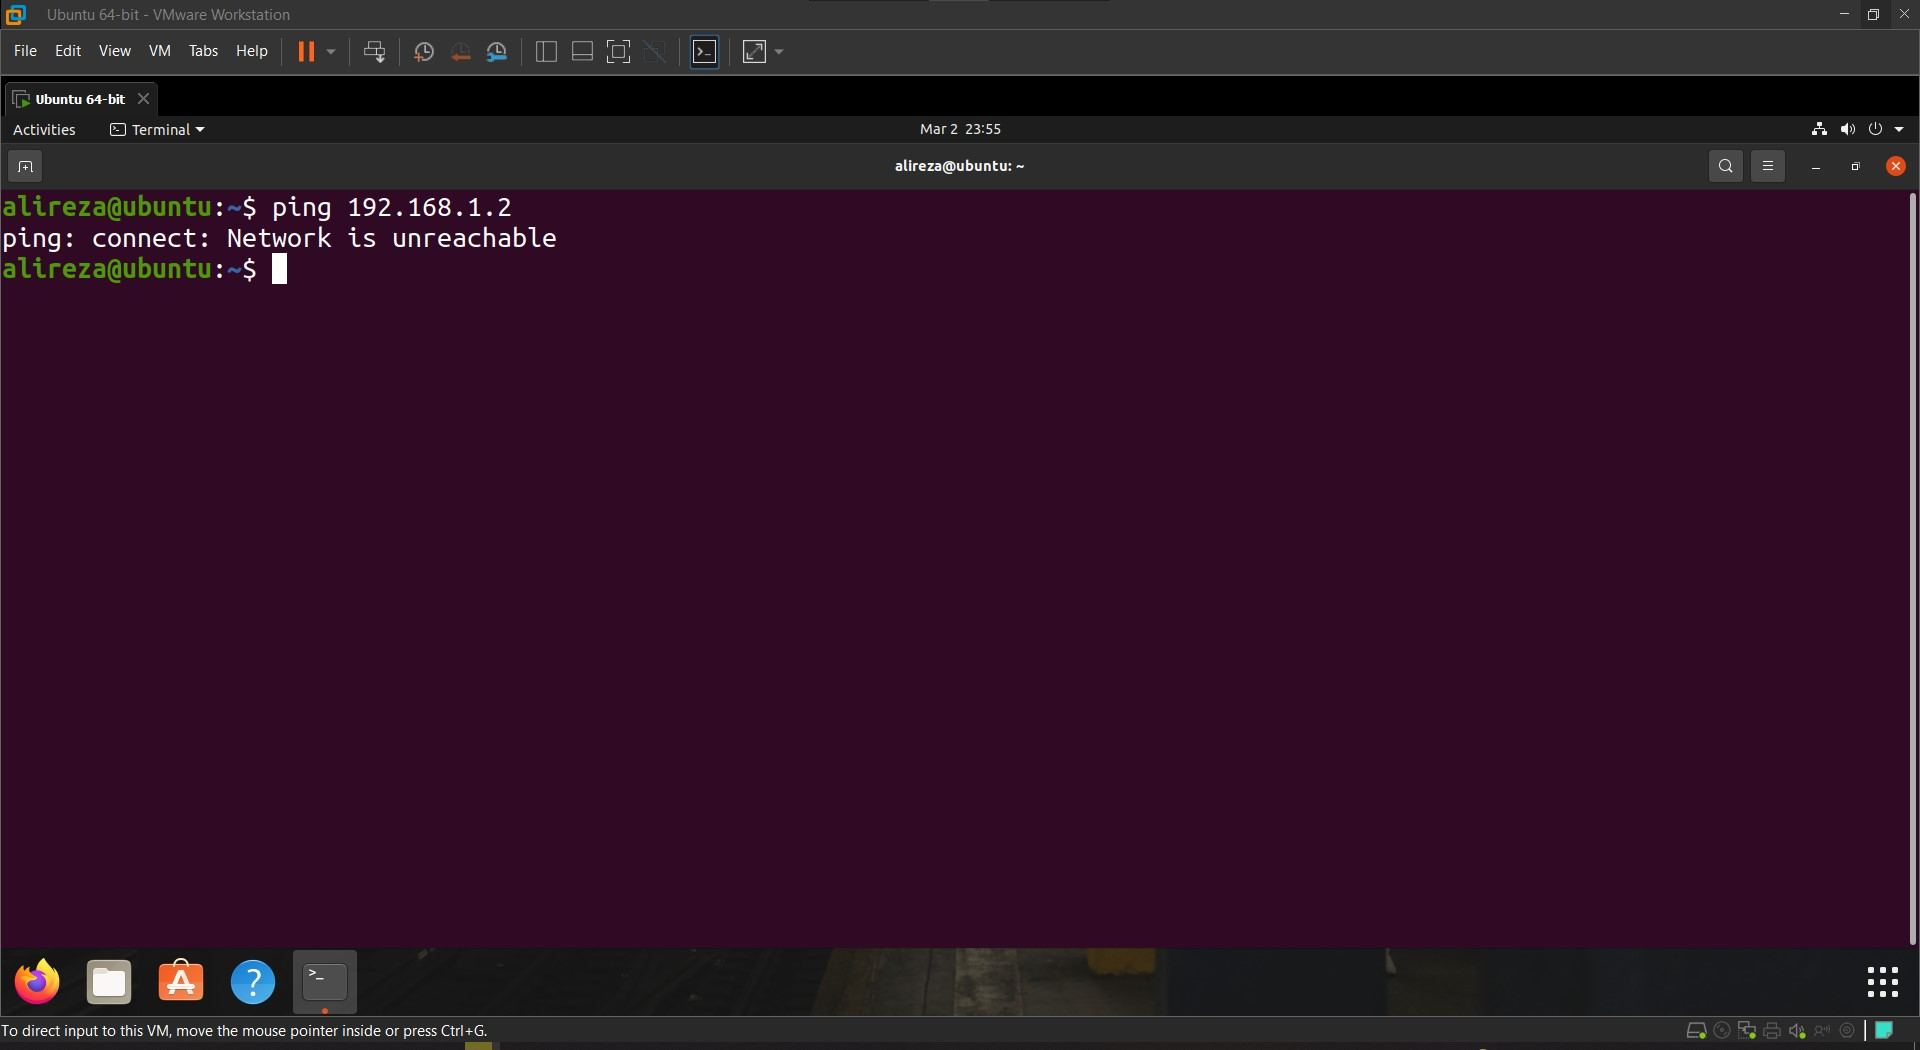
\includegraphics[width=1.0\textwidth]{figures/6b.jpg}
    \caption
	{
\lr{ping 192.168.1.2}
	}
    \label{fig:fig1}
\end{figure}
در این حالت چون رنج آی‌پی‌ها متفاوت است و همانند حالت \lr{NAT}، ترجمه اتفاق نمی‌افتد، سیستم مجازی به میزبان دسترسی ندارد.
\begin{figure}[H]
    \centering
    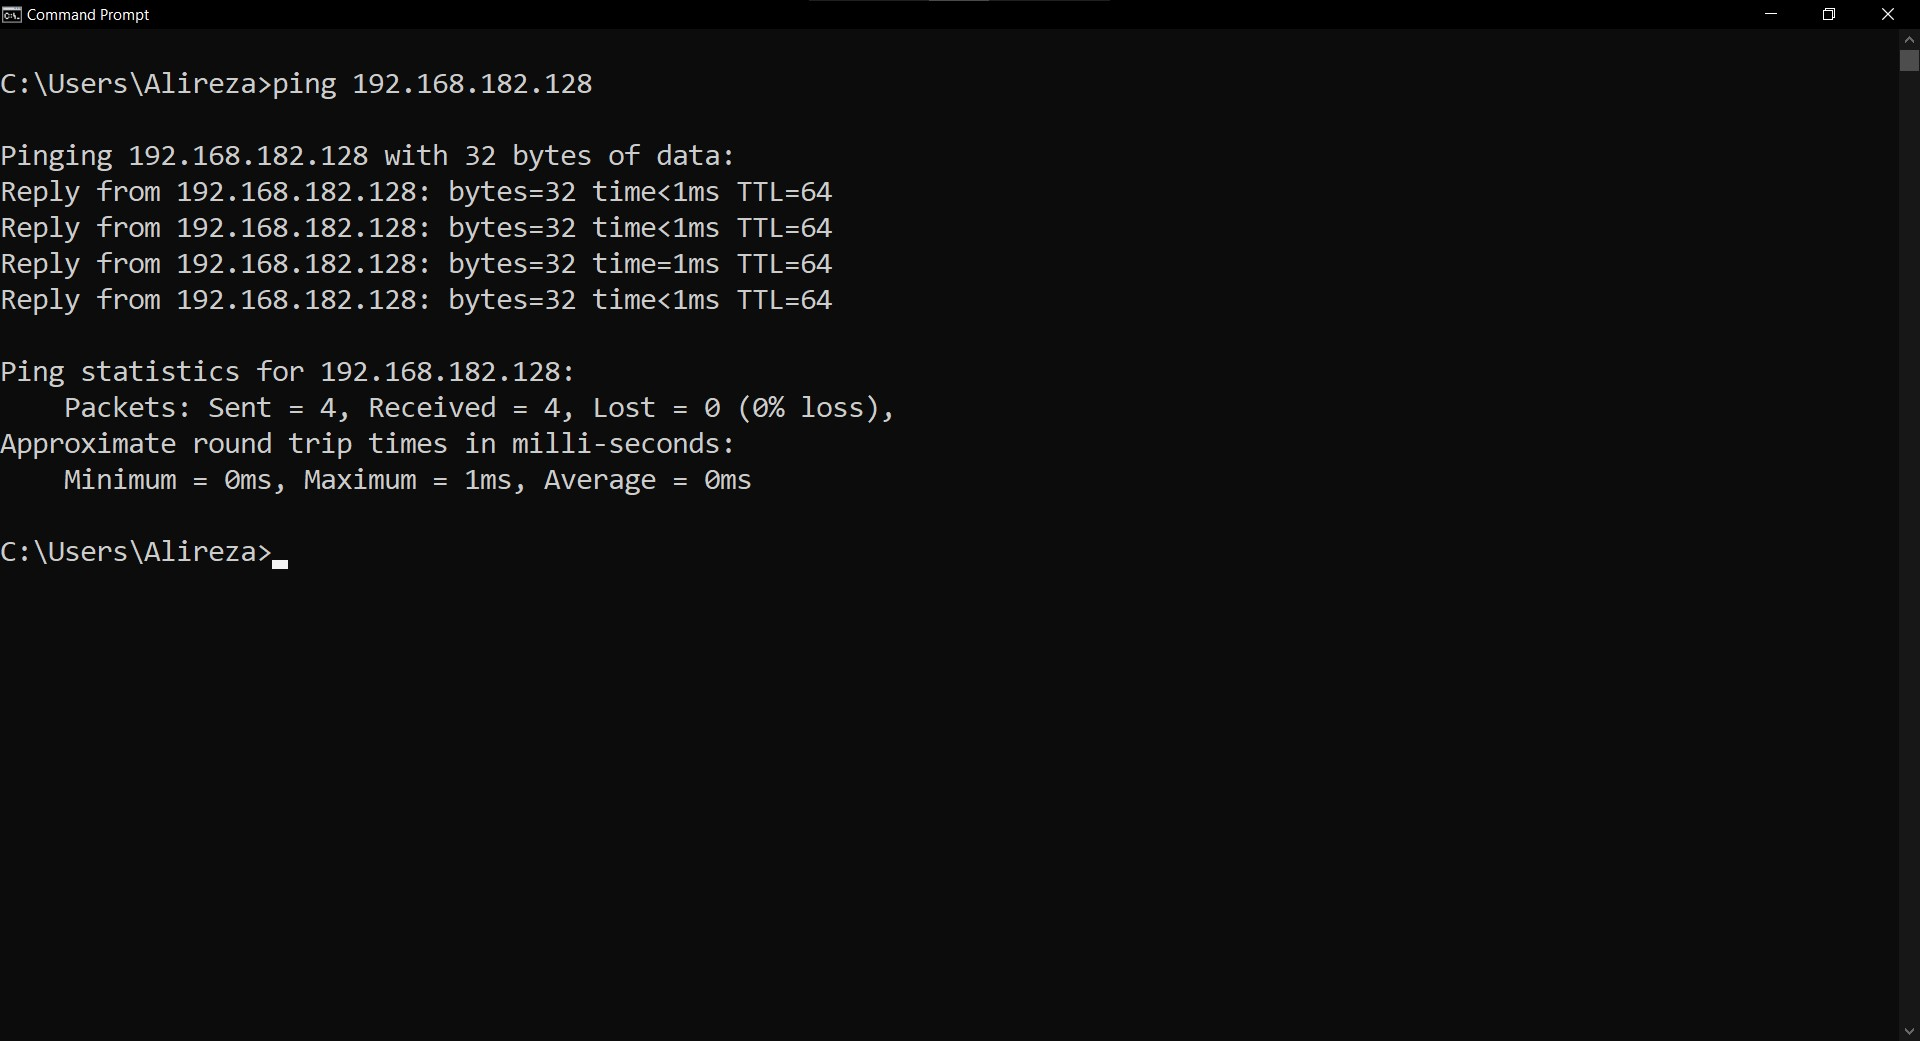
\includegraphics[width=1.0\textwidth]{figures/6c.jpg}
    \caption
	{
\lr{ping 192.168.182.128}
	}
    \label{fig:fig1}
\end{figure}
میزبان در هر سه حالت به سیستم مجازی دسترسی دارد.

\subsection{}
در حالت \lr{Bridged} ماشین مجازی از طریق کارت شبکه سیستم اصلی به شبکه محلی متصل می‌شود. در این روش کارت شبکه مجازی در ماشین مجازی به کارت شبکه فیزیکی متصل شده و می‌تواند ماشین مجازی را همانند یک سیستم مستقل به شبکه محلی متصل نماید. در صورتی که در سیستم اصلی چند کارت شبکه وجود داشته باشد، در ماشین(های) مجازی می‌توان هر کارت شبکه مجازی را با هرکدام از کارت شبکه‌های سیستم اصلی \lr{Bridge} نمود. در این حالت باید آدرس آی‌پی‌های ماشین مجازی و کارت شبکه فیزیکی که با آن \lr{Bridge} شده است در یک رنج باشند تا بتوانند ارتباط لایه 2 درستی با یکدیگر برقرار نمایند. در مجموع می‌توان گفت در این حالت ماشین مجازی همانند یک ماشین مستقل در شبکه محلی دیده می‌شود و در صورتی که ارتباط اینترنت در شبکه محلی وجود داشته باشد ماشین مجازی نیز می‌تواند به شبکه متصل شود. در شکل زیر نحوه ارتباط در این مدل نشان داده شده است.
\begin{figure}[H]
    \centering
    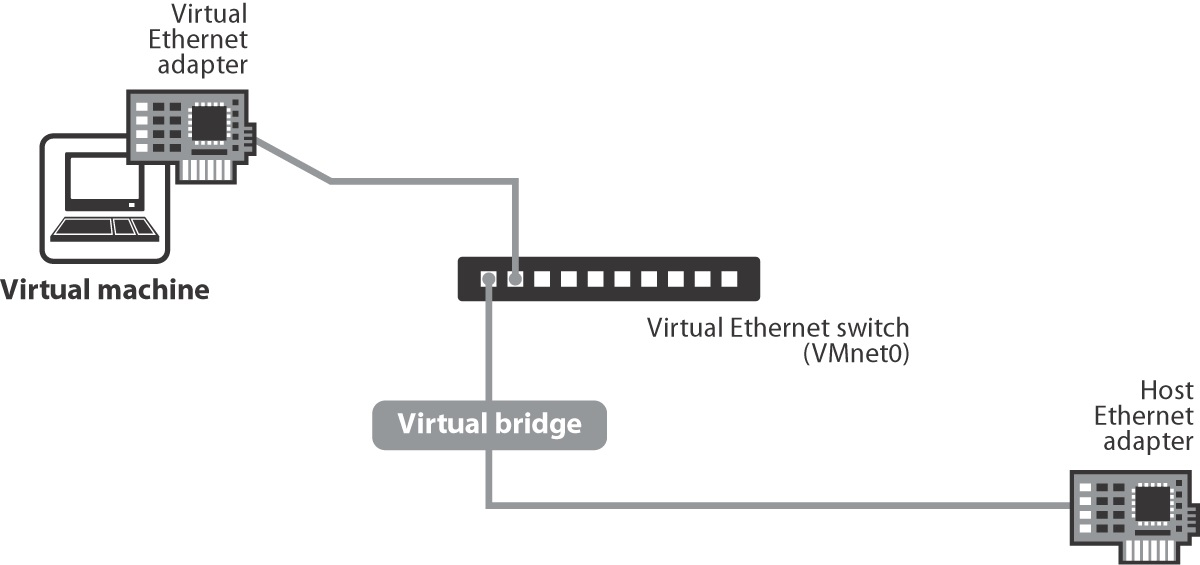
\includegraphics[width=1.0\textwidth]{figures/7a.jpg}
    \caption
	{
\lr{Bridged}
	}
    \label{fig:fig1}
\end{figure}
در حالت \lr{Host-only} کارت شبکه‌ی مجازی به \lr{VMnet1} متصل می‌شود. در این حالت با
توجه به تنظیماتی که در \lr{VMnet1} اعمال شده است. \lr{DHCP server} به کارت شبکه مجازی
یک آی‌پی از رنج مشخص شده اختصاص می‌دهد و ماشین‌های مجازی که کارت شبکه آن ها به \lr{VMnet1} متصل شده است. می‌توانند با یکدیگر ارتباط برقرار نمایند. درحالت \lr{Host-only} با توجه به این که مشخصه فیزیکی در سوییج مجازی \lr{VMnet1} وجود ندارد، نمی‌توان به اینترنت و یا دنیای بیرون \lr{Host} متصل شد. در شکل زیر ساختار این حالت نشان داده شده است.
\begin{figure}[H]
    \centering
    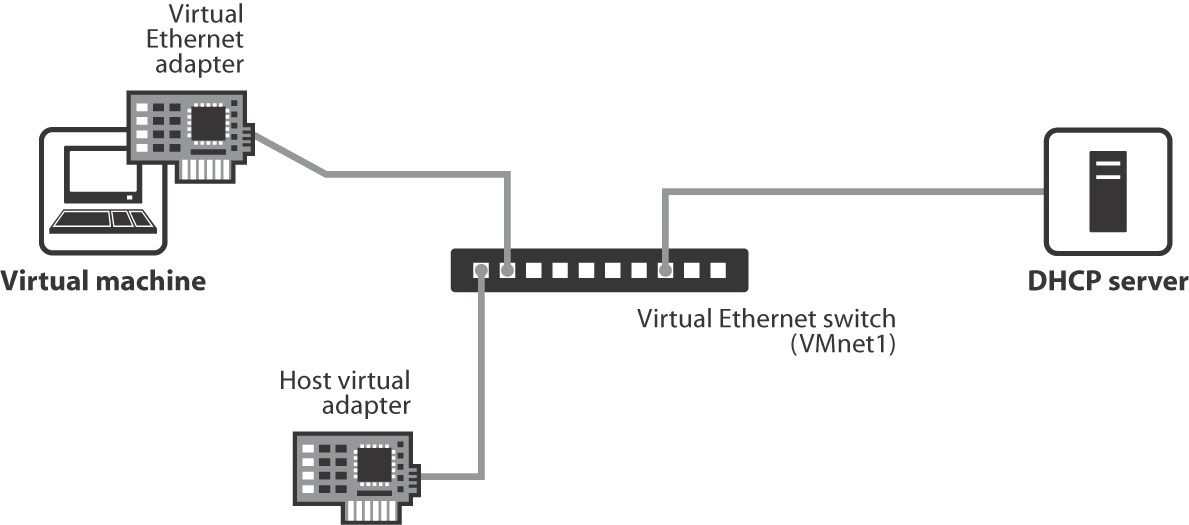
\includegraphics[width=1.0\textwidth]{figures/7b.jpg}
    \caption
	{
\lr{Host-only}
	}
    \label{fig:fig1}
\end{figure}
در حالت \lr{NAT} کارت شبکه‌ی مجازی از رنج آدرس آی‌پی‌های اختصاص داده شده به \lr{VMnet8} آدرس آی‌پی دریافت می‌کند و در صورتی که ترافیک ماشین مجازی بخواهد بیرون رود، با آدرس ماشین اصلی \lr{NAT} می‌شود و آن‌گاه بیرون می‌رود.در شکل زیر ساختار این حالت نشان داده شده است.
\begin{figure}[H]
    \centering
    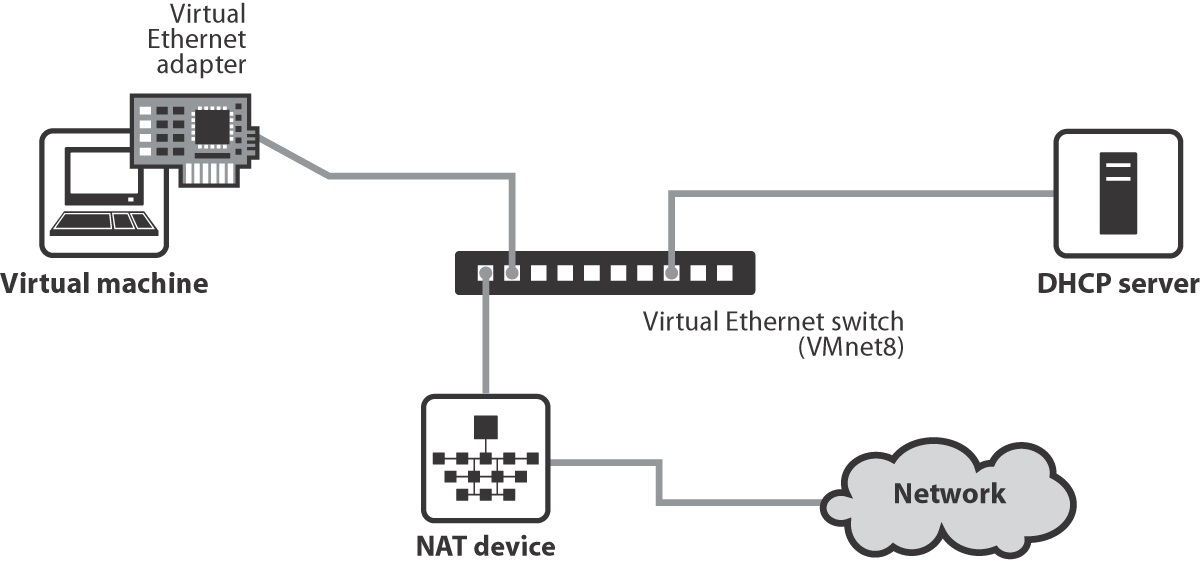
\includegraphics[width=1.0\textwidth]{figures/7c.jpg}
    \caption
	{
\lr{NAT}
	}
    \label{fig:fig1}
\end{figure}

\subsection{}
\begin{figure}[H]
    \centering
    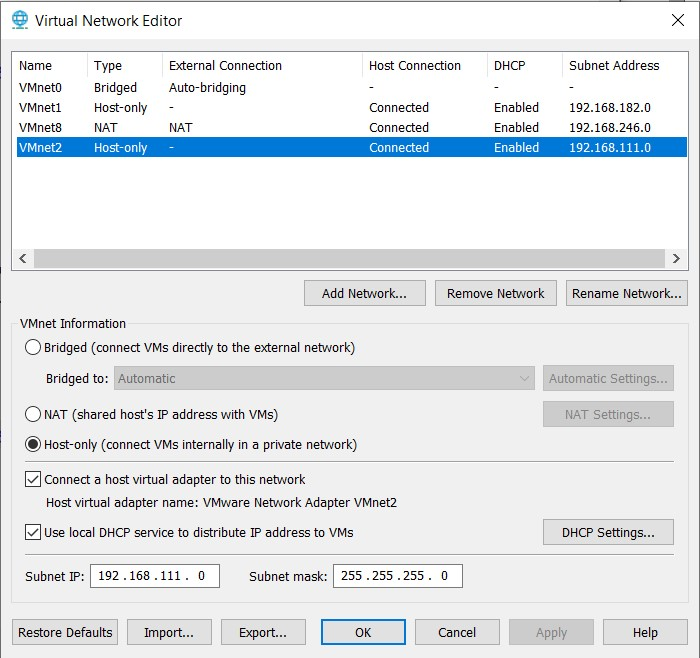
\includegraphics[width=1.0\textwidth]{figures/8a.jpg}
    \caption
	{
\lr{Virtual Network Editor(VMnet2)}
	}
    \label{fig:fig1}
\end{figure}

\begin{figure}[H]
    \centering
    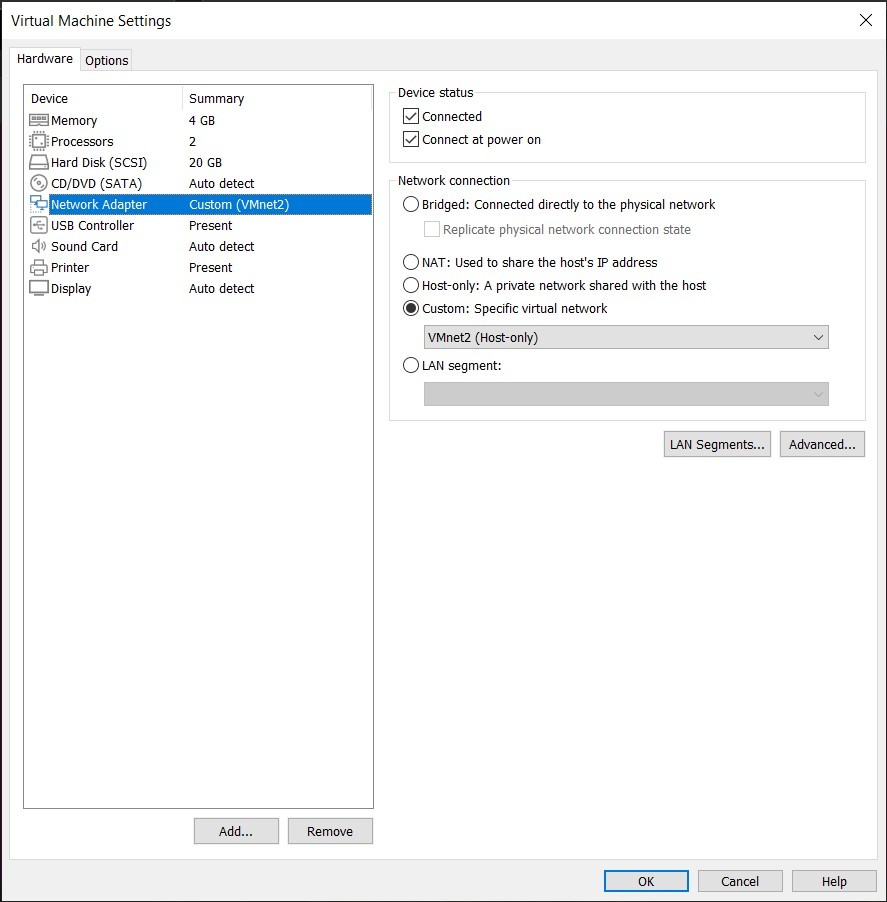
\includegraphics[width=1.0\textwidth]{figures/8b.jpg}
    \caption
	{
\lr{Virtual Machine Setting(Custom)}
	}
    \label{fig:fig1}
\end{figure}

\begin{figure}[H]
    \centering
    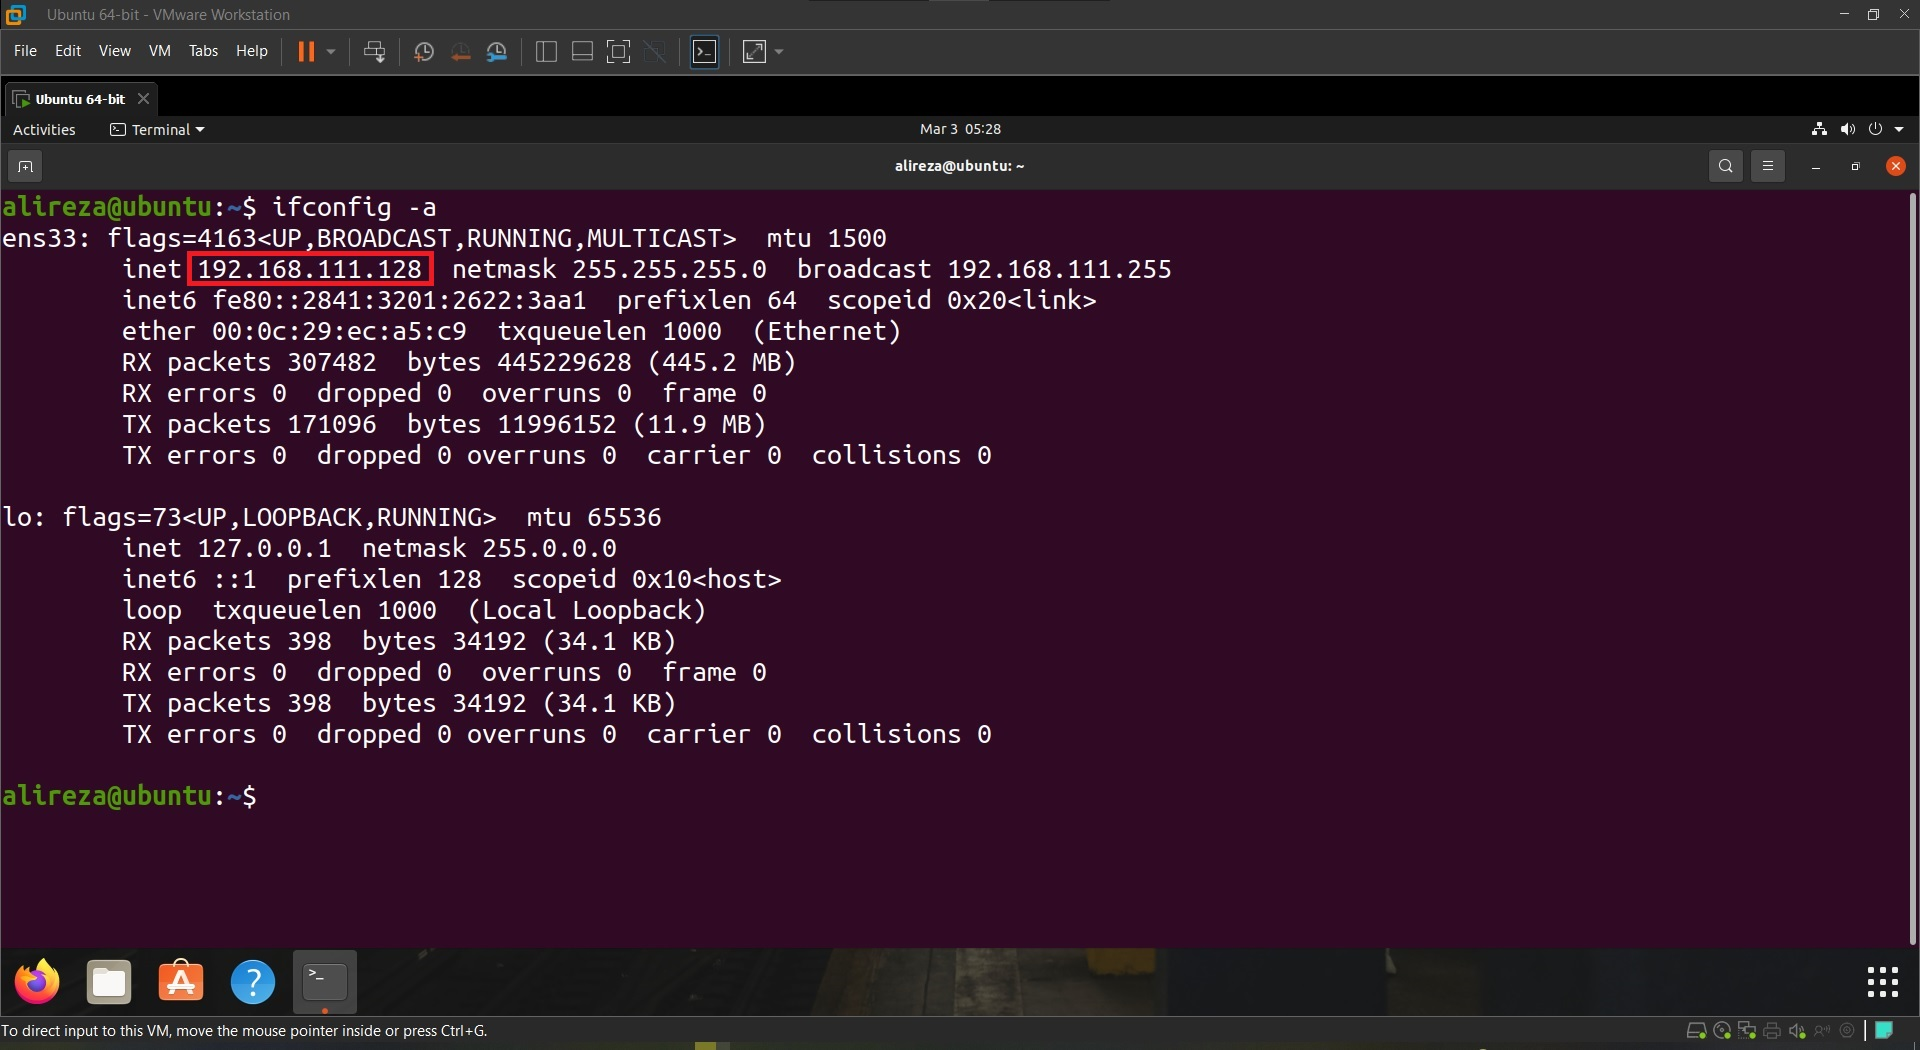
\includegraphics[width=1.0\textwidth]{figures/8c.jpg}
    \caption
	{
\lr{ifconfig -a}
	}
    \label{fig:fig1}
\end{figure}
همانطور که می‌بینیم آدرس دریافت شده در همان محدوده‌ای است انتظار داشتیم و برابر \lr{192.168.111} است.

\subsection{}
\begin{figure}[H]
    \centering
    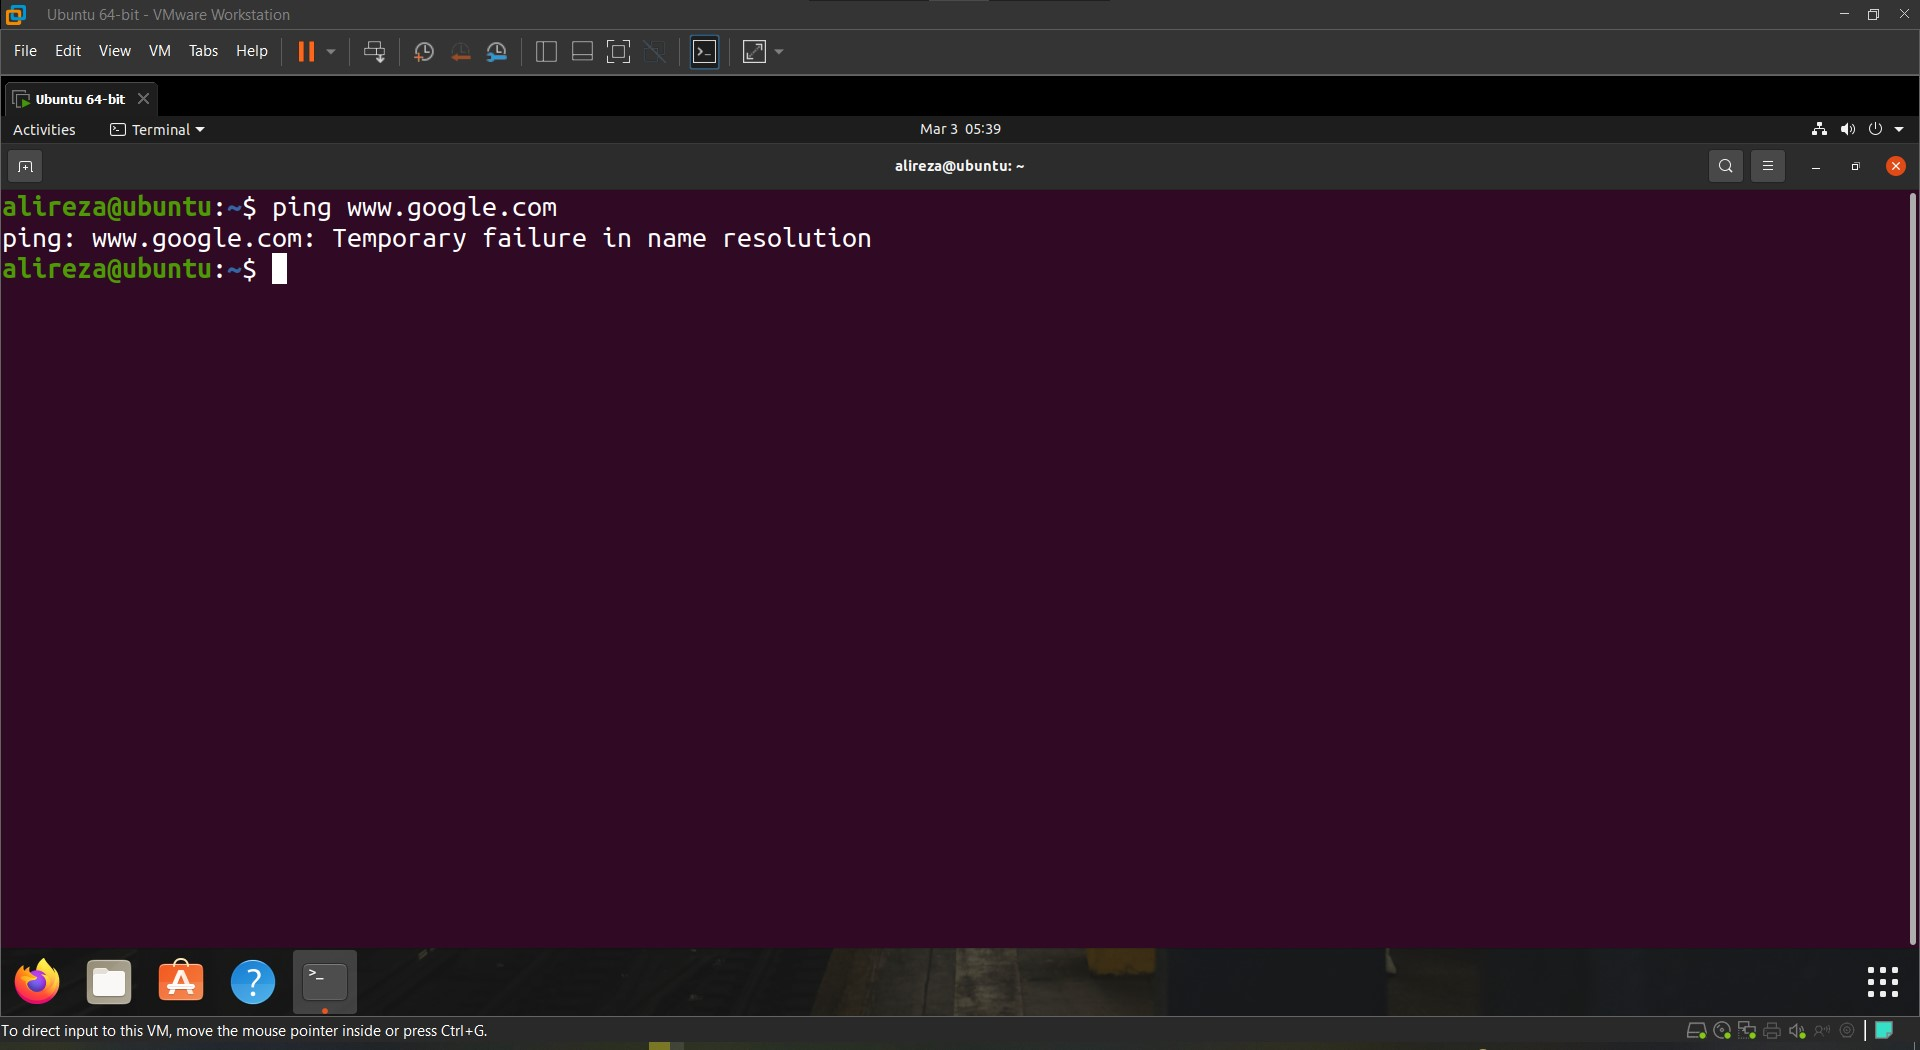
\includegraphics[width=1.0\textwidth]{figures/9a.jpg}
    \caption
	{
\lr{ping www.google.com -c 3}
	}
    \label{fig:fig1}
\end{figure}

\begin{figure}[H]
    \centering
    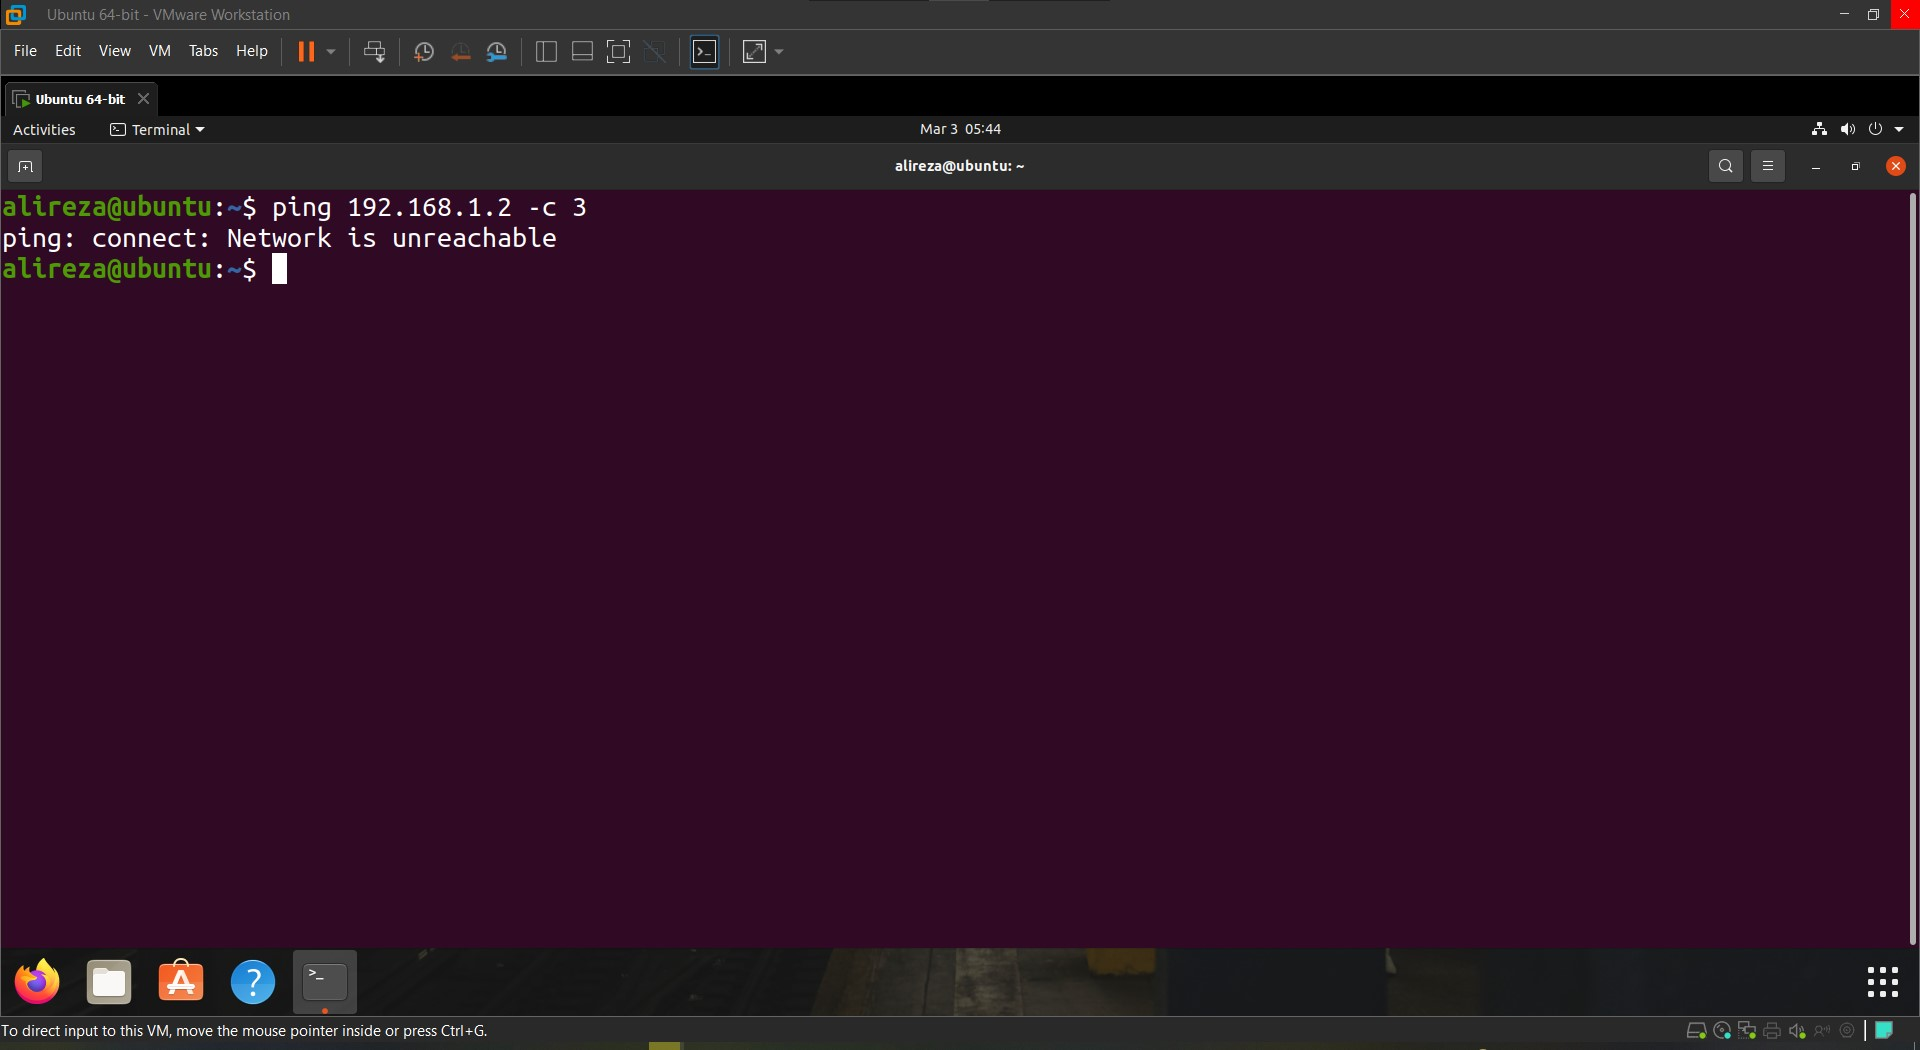
\includegraphics[width=1.0\textwidth]{figures/9b.jpg}
    \caption
	{
\lr{ping 192.168.1.2 -c 3}
	}
    \label{fig:fig1}
\end{figure}
چون اتصال در حالت \lr{Host-only} است پس نه به اینترنت دسترسی دارد و نه به میزبان.

%چون در حالت \lr{NAT} در صورتی که ترافیک ماشین مجازی بخواهد بیرون رود، با آدرس ماشین اصلی \lr{NAT} می‌شود و آن‌گاه بیرون می‌رود، با آنکه 

%%%%%%%%%%%%%%%%%%%%%%%%%%%%%%%%%%%%%%%%%%%%%%

\section*{منابع}
\renewcommand{\section}[2]{}%
\begin{thebibliography}{99} % assumes less than 100 references
%چنانچه مرجع فارسی نیز داشته باشید باید دستور فوق را فعال کنید و مراجع فارسی خود را بعد از این دستور وارد کنید


\begin{LTRitems}

\resetlatinfont

\bibitem{b1} 
\end{LTRitems}

\end{thebibliography}


\end{document}
